\documentclass[10pt,a4paper]{article}
\usepackage[utf8]{inputenc}
\usepackage{amsmath}
\usepackage{amsfonts}
\usepackage{amssymb}
\usepackage{graphicx}
\usepackage{subcaption}
\graphicspath{{Pictures/}}
\usepackage{hyperref}
\usepackage{listings}
\usepackage{framed}
\usepackage{pdfpages}
\usepackage{appendix}
\addtolength{\oddsidemargin}{-.875in}
\addtolength{\evensidemargin}{-.875in}
\addtolength{\textwidth}{1.75in}

\addtolength{\topmargin}{-.875in}
\addtolength{\textheight}{1.75in}


\begin{document}
\title{Tutorial for the installation of Outer tracker hybrid test system}
\author{P. Chatagnon, F. Ferro}
\date{\today} 

\maketitle

All the instructions below can be found at the following links:
\begin{itemize}
\item  \url{https://cms-tracker-daq.web.cern.ch/cms-tracker-daq/} : All information on how to connect the FC7, upload firmwares, etc
\item  \url{https://gitlab.cern.ch/cms_tk_ph2/Ph2_ACF} : Repository for the acquisition software
\item  \url{https://gitlab.cern.ch/cms_tk_ph2/cmsph2_tcusb} : library handling the usb communication between the PC and the crate
\end{itemize}

\section{Overview of the test system}

This tutorial describes the steps to install the hybrid test system for the Phase 2 tracker of CMS. A schematic description of the test system is shown in Figure \ref{TestSchematic}. The following instructions describe the installation of the connections between the PC and the multiplexing crate, the PC and the FC7 and the power supply of the crate. 
\begin{figure}[h!]
 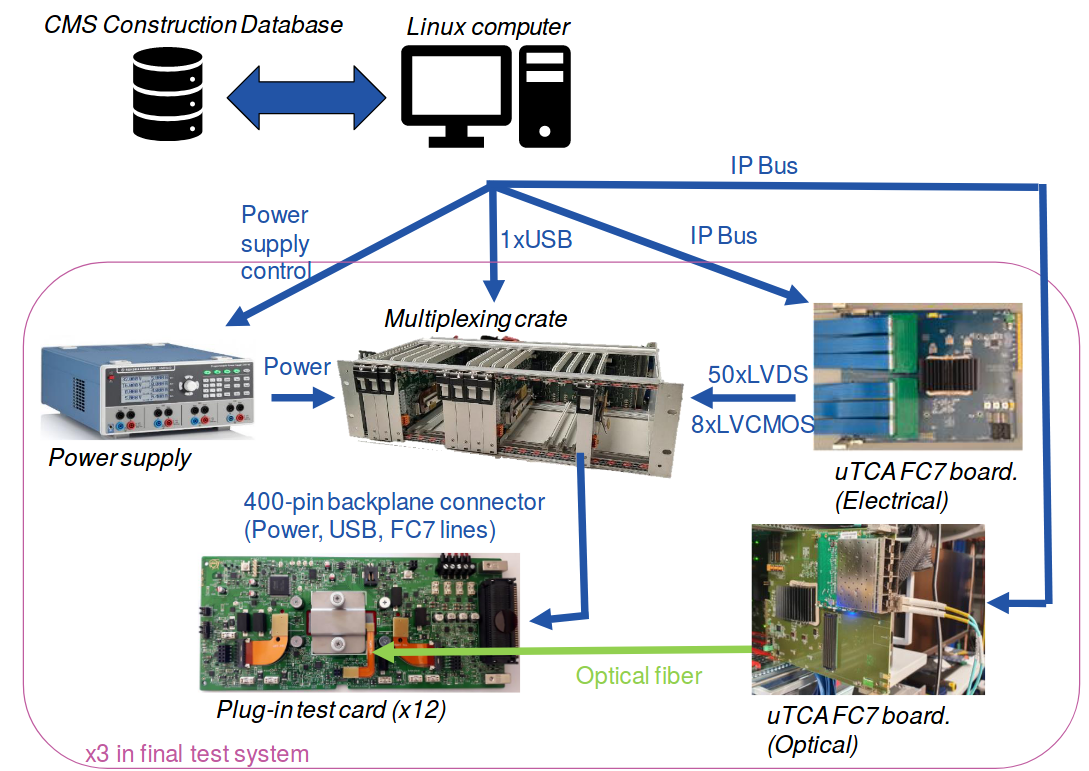
\includegraphics[width=\linewidth]{TestOverview.png} 
  \caption{Scheme of the complete test system}
  \label{TestSchematic}
\end{figure}

Figure \ref{PhotoTestSystem} shows the test system installed in Genova. The FC7 are hosted in the uTCA (top of the picture). The test crate is visible in the bottom of the picture.

\begin{figure}[h!]
\centering
 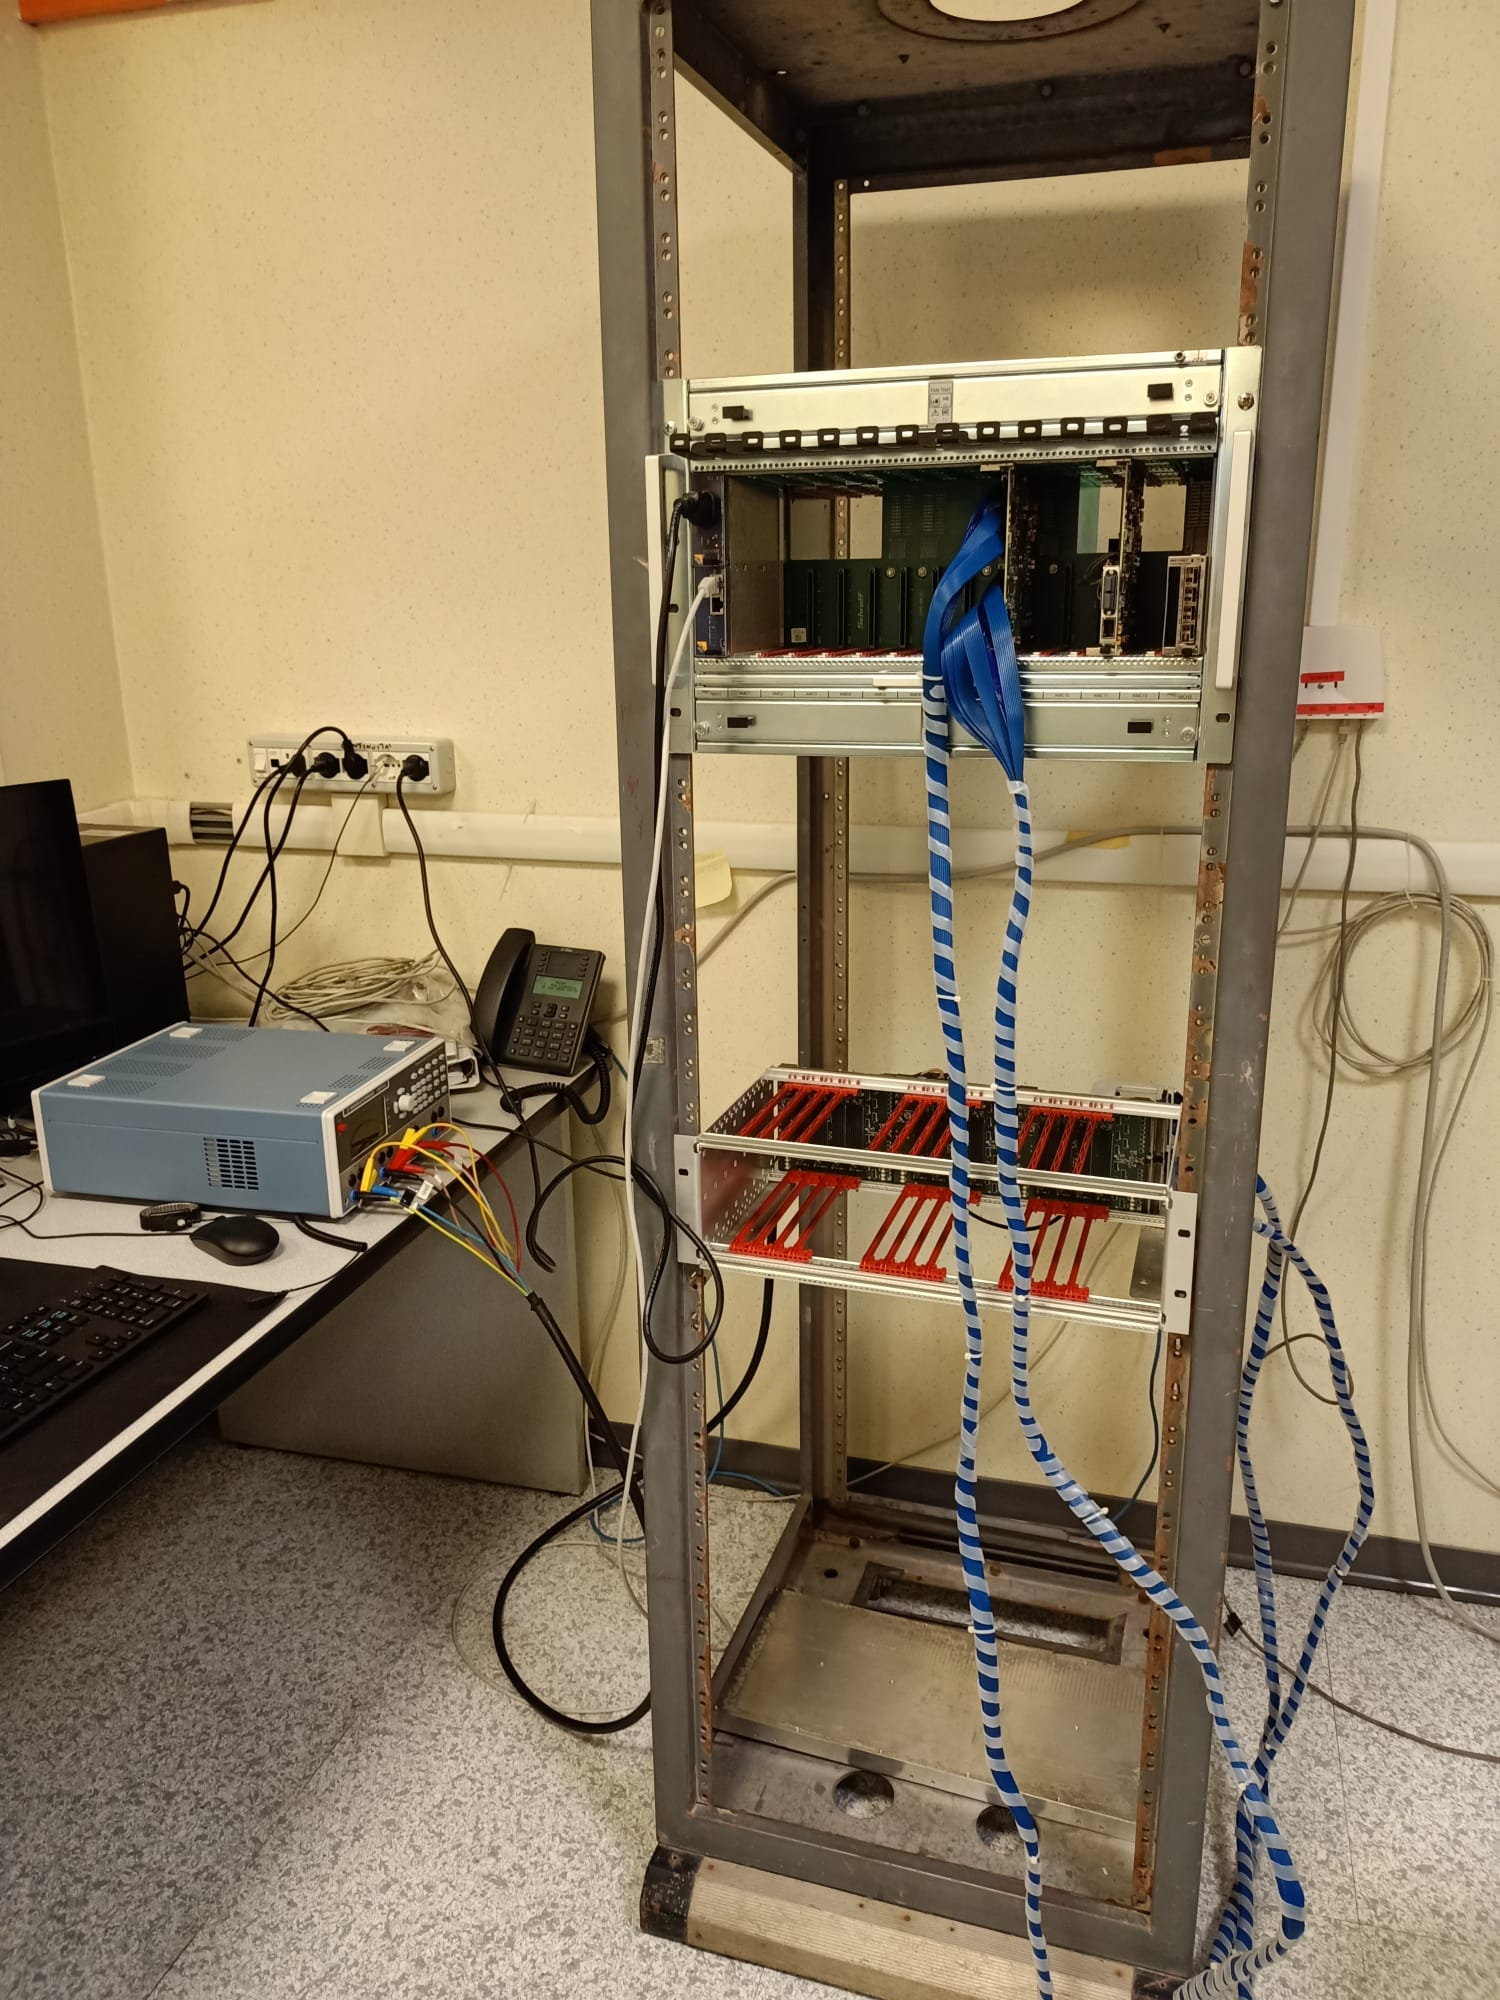
\includegraphics[width=0.5\linewidth]{TestSystem.jpeg} 
  \caption{Overview of the test system in Genova}
  \label{PhotoTestSystem}
\end{figure}

\section{Hardware}
In this section the steps to install the various hardware parts of the system are detailed.
\subsection{Power cabling and power supply setting}
The test crate is powered by a \emph{ROHDE\&SCHARTZ HMP4040} power supply. The power cable is connected following the schematic of Figure \ref{PowerConnection}. The various power cables are clearly labeled as shown in Figure \ref{PhotoPowerConnection}.
\begin{figure}[h!]
\centering
 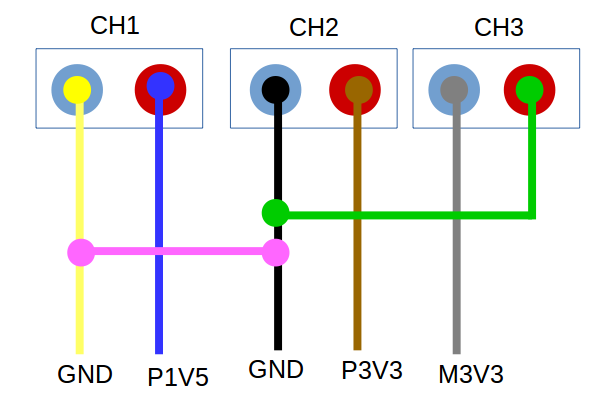
\includegraphics[width=0.7\linewidth]{ElectricalPower.png} 
  \caption{Schematic display of the connection of the crate power cable on the power supply.}
  \label{PowerConnection}
\end{figure}

\begin{figure}[h!]
\centering
 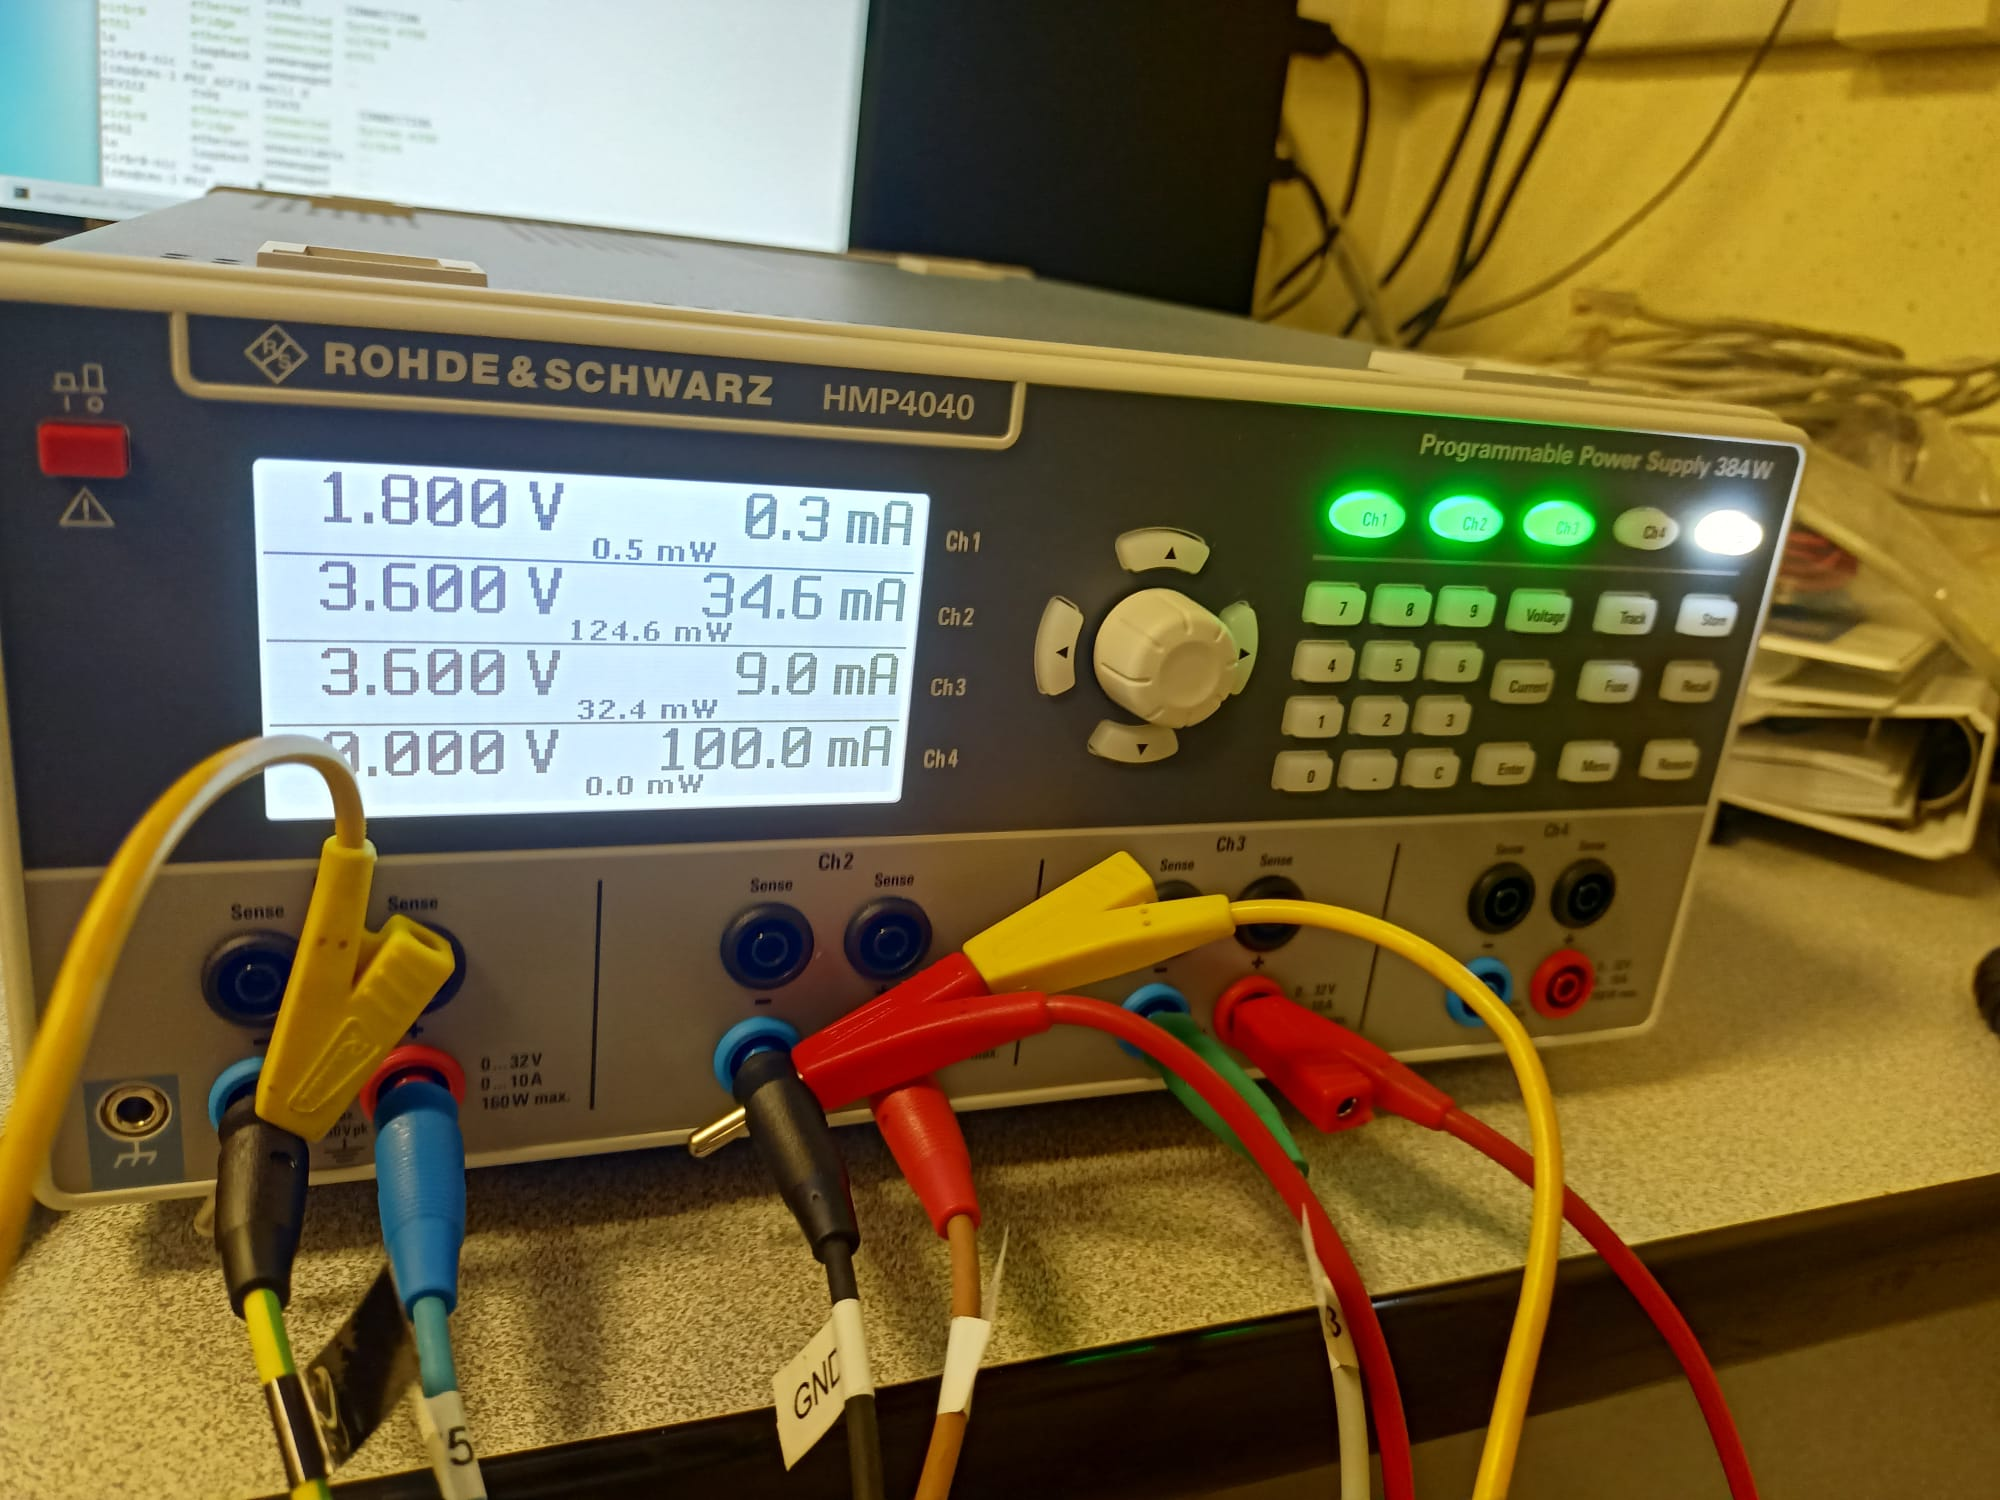
\includegraphics[width=0.7\linewidth]{PowerSupply.jpeg} 
  \caption{Fully configured power supply.}
  \label{PhotoPowerConnection}
\end{figure}

The voltages and current limit have to be set as indicated in Table \ref{tableV}. Once the voltage and current are set, the cable can be plugged in the back of the crate in any power plug, as shown in Figure \ref{PhotoPowerConnectionCrate}.
The cable connections for the test of ROH and POH's are the same. Channel1 has a fixed voltage for ROH tests while for POH's it becomes a {\it Test channel} and its voltage is remotely controlled. Note that, in the case of POH test, if the starting voltage of Channel1 is not set to 10.5V the test card cannot be configured.  
\par The ethernet card of the PS must be correctly configured, proving a fixed IP address. It has to be in the same subnet as for the FC7's - see section \ref{fc7connection} ({\it in our case: 192.168.0.10}).

\begin{figure}[h!]
\centering
 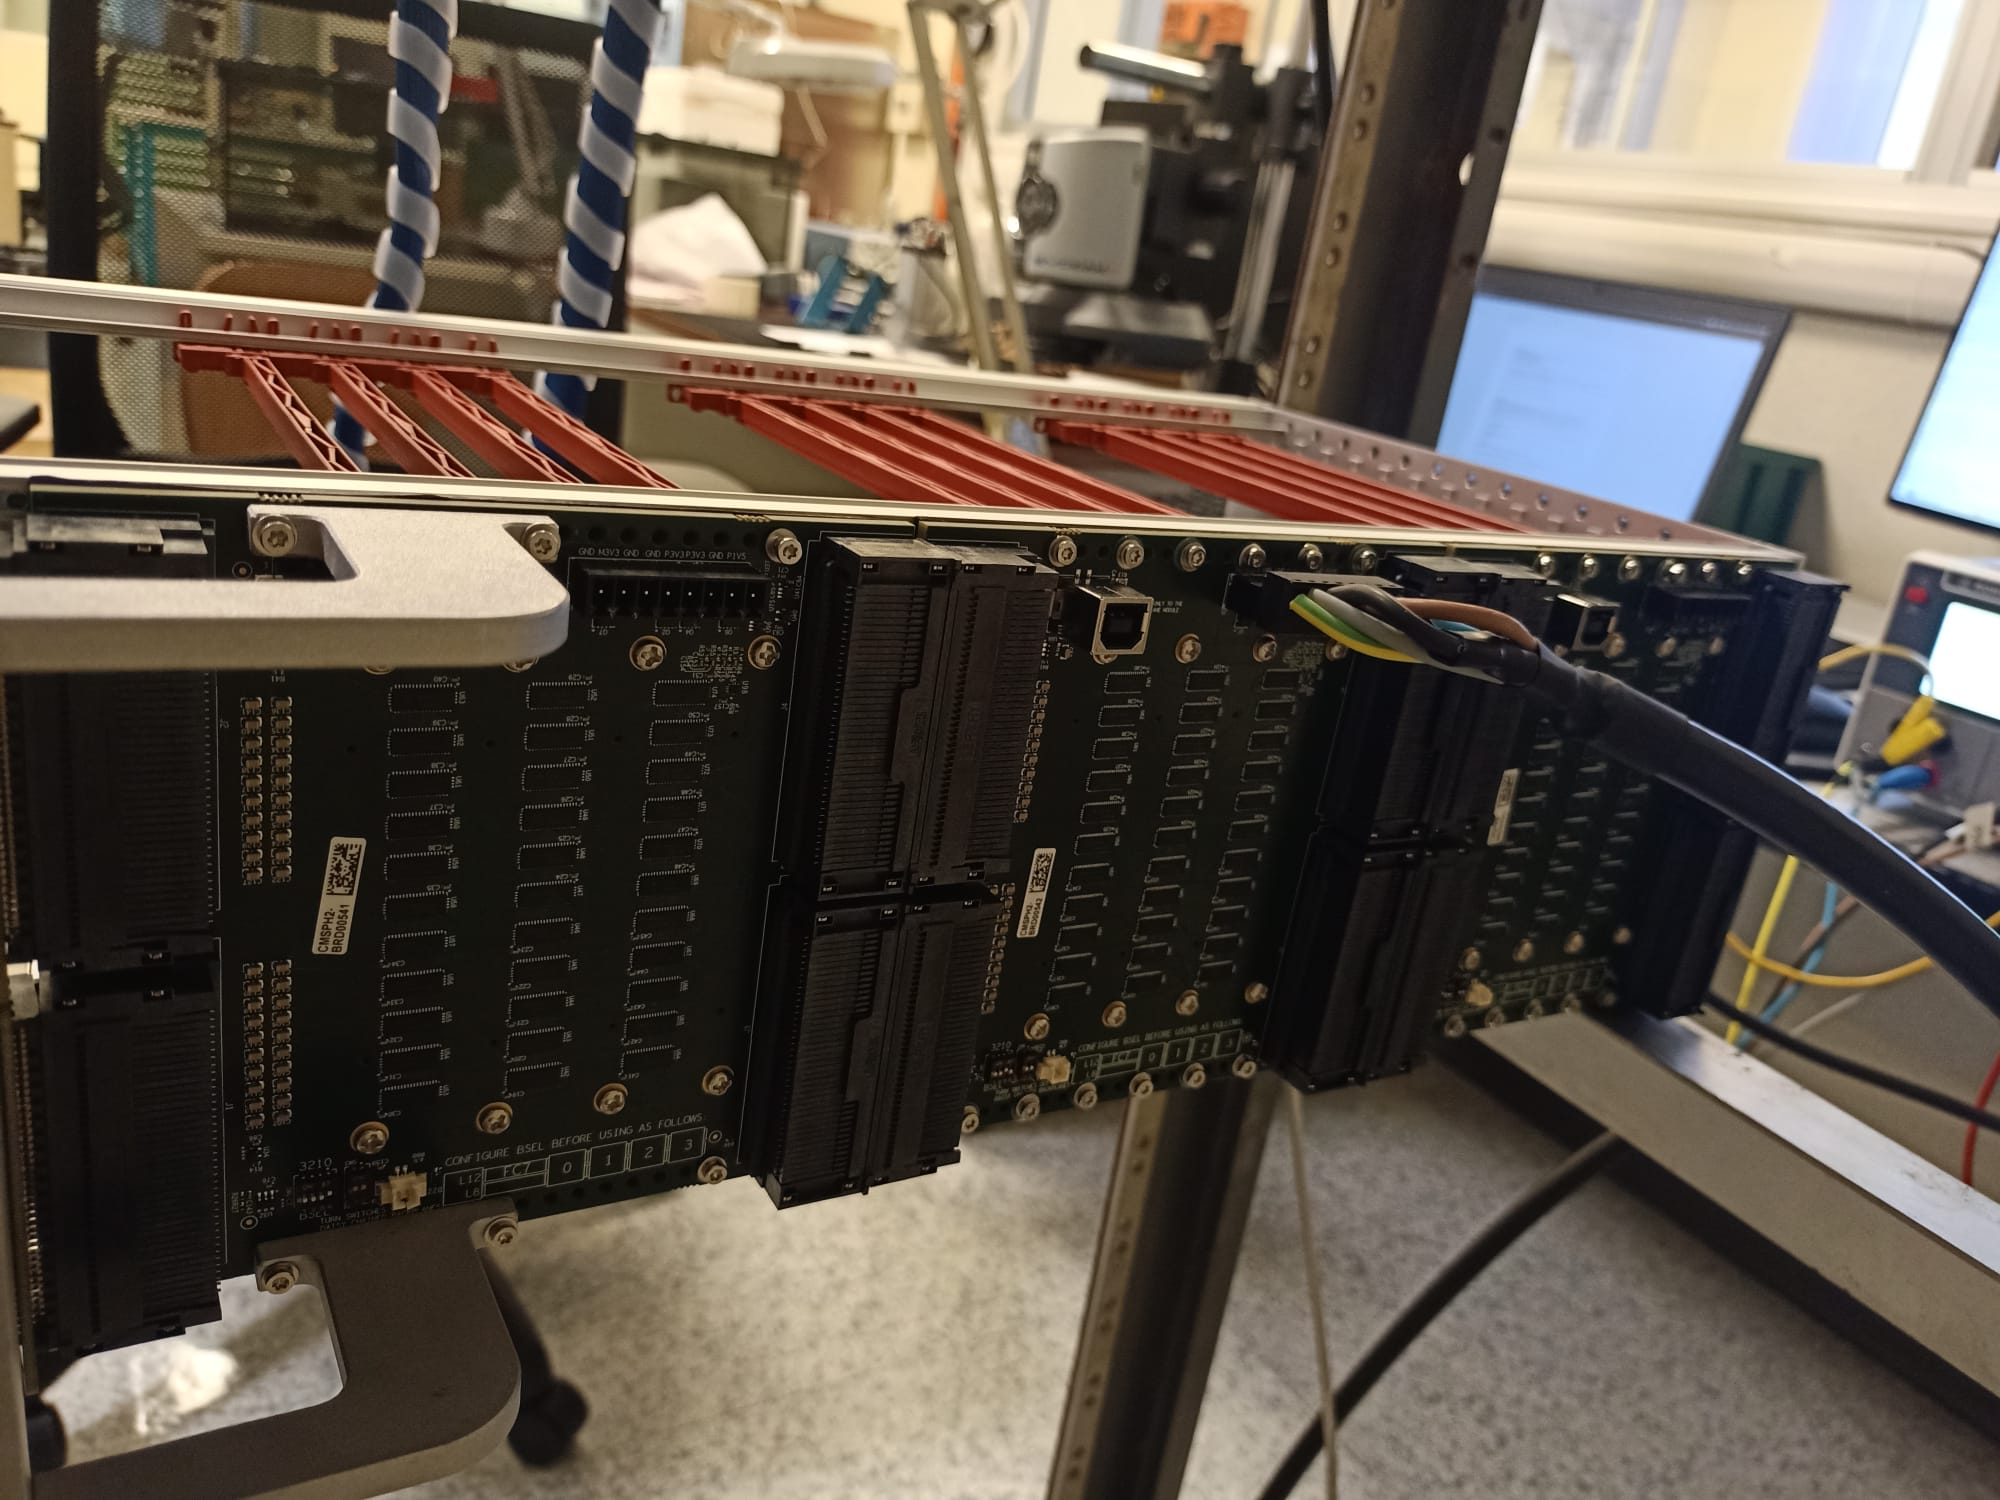
\includegraphics[width=0.7\linewidth]{PowerCable.jpeg} 
  \caption{Picture showing the power cable connection to the crate. The cable can be plugged in any of the three backplanes (here it is on the middle one).}
  \label{PhotoPowerConnectionCrate}
\end{figure}

\begin{table}[h!]
\centering
\begin{tabular}{|c|c|c|c|}
\hline 
Channel & CH1 & CH2 & CH3 \\ 
\hline 
Pair & P1V5 & P3V3 & M3V3 \\ 
\hline 
V (ROH)& 1.8 V & 3.5 V & 3.6 V \\
V (POH)& 10.5 V & 3.5 V & 3.6 V \\
$A_{max}$ & 2 A & 4 A & 1 A \\ 
\hline 
\end{tabular} 
\label{tableIV}
\caption{Voltage and current limit to apply to each channel of the power supply}
\end{table}

\subsection{Backplanes setting}
In order for the test card multiplexing to work, each backplane has to be given a unique adress. This is possible using physical switches located on the back of every backplanes. The switches are located as shown on Figure \ref{BackPlaneSwitch}. Each switch corresponds to a unique address from 0 to 3 and is activated when in its upward position. The addressing of each backplane must be done in the following way: the backplane hosting the FMC connections must be addressed 0, the following one 1, and the furthest from the FMC connector 2.

\begin{figure}[h!]
 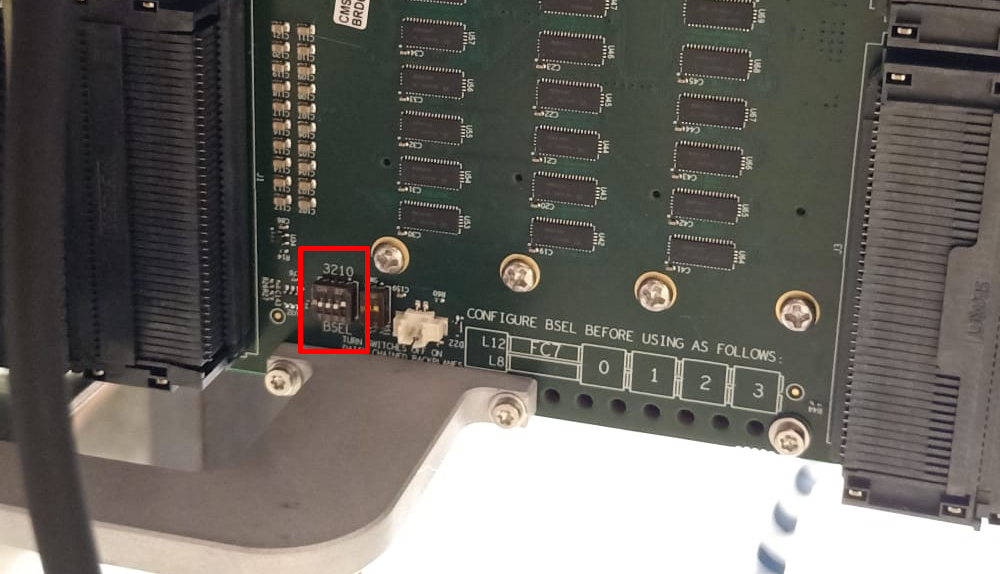
\includegraphics[width=\linewidth]{BackPlaneSwitch.jpeg} 
  \caption{Switches used to provide a physical address to each backplane of a crate. The address corresponding to each switch is printed above each one of them, in this case the address is 0 corresponding to the backplane with the FMC connections to the FC7.}
  \label{BackPlaneSwitch}
\end{figure}

\subsection{Data transmission cables}
Once the power cable is correctly installed, the FMCs and usb cables have to be installed.
\subsubsection{FMC cables connections}
Two FMC cables link the test crate with the FC7 used to control the backplanes. The FC7 have two FMC connectors denoted L12 and L8, while the backplane connectors are denoted J1 and J2. The FMC cables have to be plugged as:
\begin{itemize}
\item L8 $\rightarrow$ J2
\item L12 $\rightarrow$ J1.
\item i.e. the upper part of the FC7 connected with the lower part of the mini-crate.
\end{itemize}
The blue flat canles should be connected to the backplane (bp) 0, as well as the USB cable. 

Schematically the FMC connections are shown in Figure \ref{FMCConnection}.
\begin{figure}[h!]
 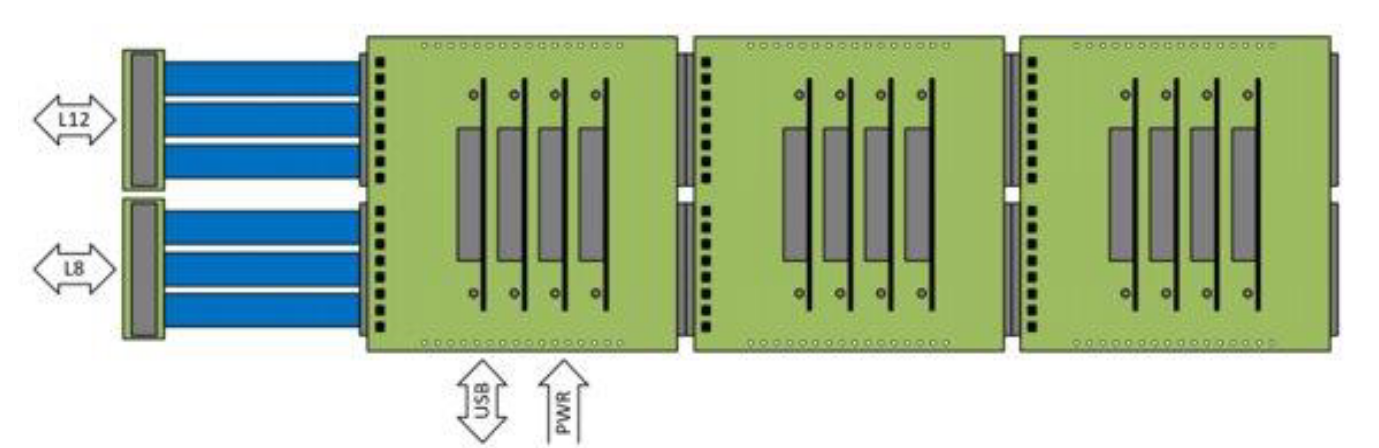
\includegraphics[width=\linewidth]{FMCScheme.png} 
  \caption{FMC Connection scheme}
  \label{FMCConnection}
\end{figure}

On both the FC7 and on the crate, the cables are secured using metallic pieces screwed in place. They can be seen on Figure \ref{FMC_FC7} and \ref{FMC_Crate}. Finally, note that an adaptator is needed to plug the FMC cables on the crate. They can be seen in place on Figure \ref{FMC_Crate}.

\begin{figure}[h!]
\centering
 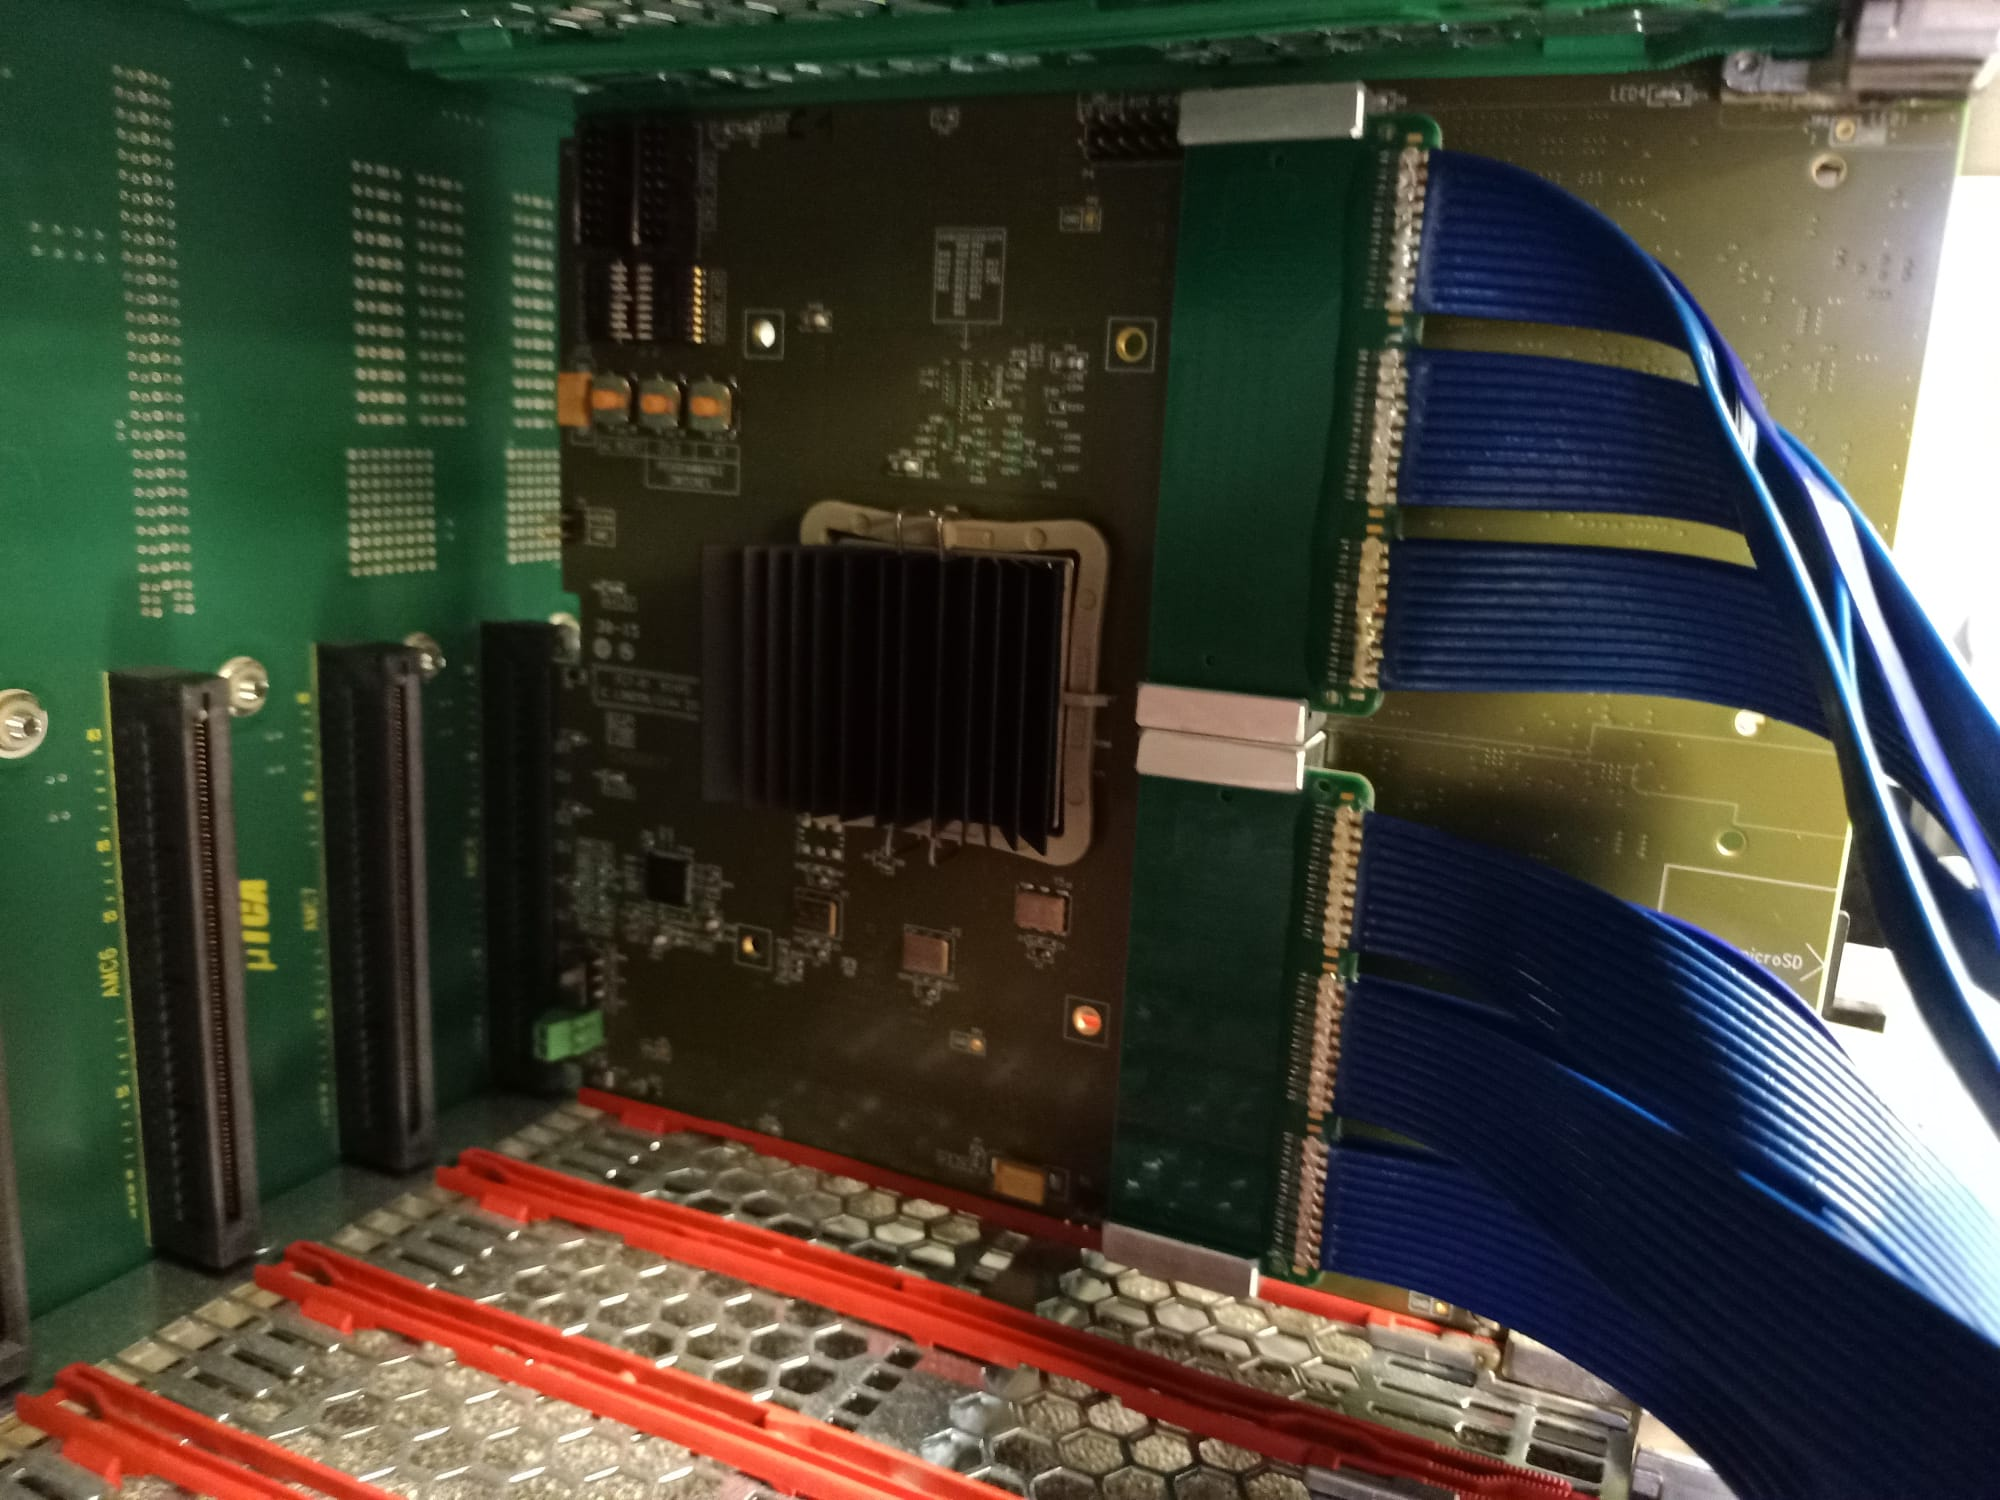
\includegraphics[width=0.6\linewidth]{FMC_FC7.jpeg} 
  \caption{Picture of the FMC cable connection on the FC7. The connection is secured using rectangular metallic pieces, visible on the picture on each side of the connectors, which are screwed directly on the FC7.}
  \label{FMC_FC7}
\end{figure}

\begin{figure}[h!]
\centering
 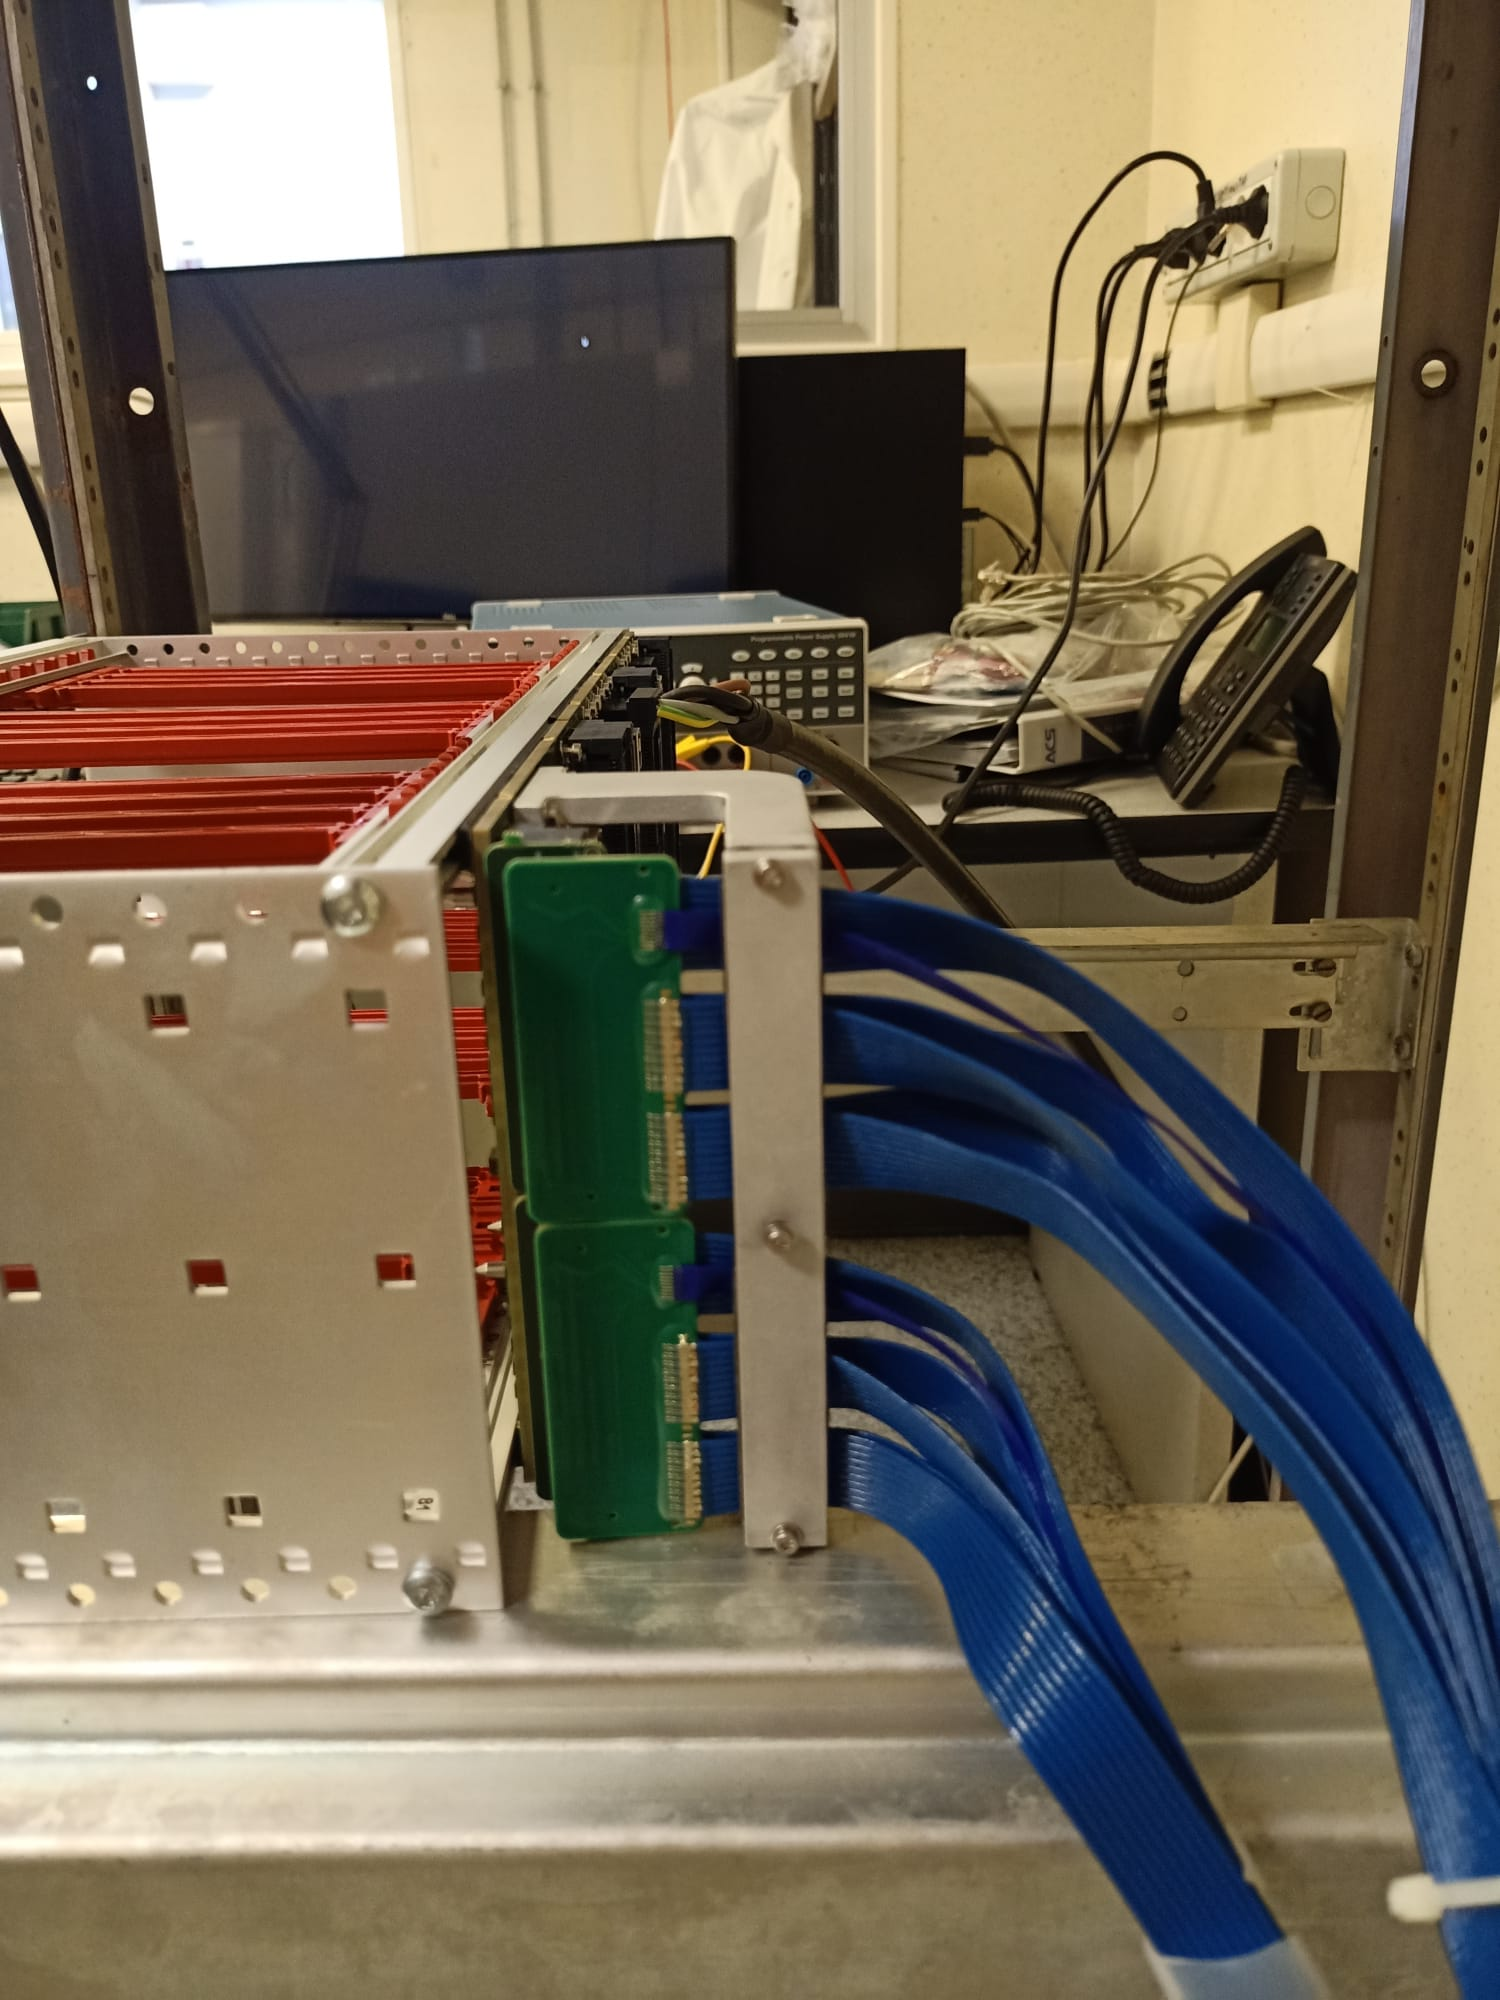
\includegraphics[width=0.4\linewidth]{FMC_Crate.jpeg} 
 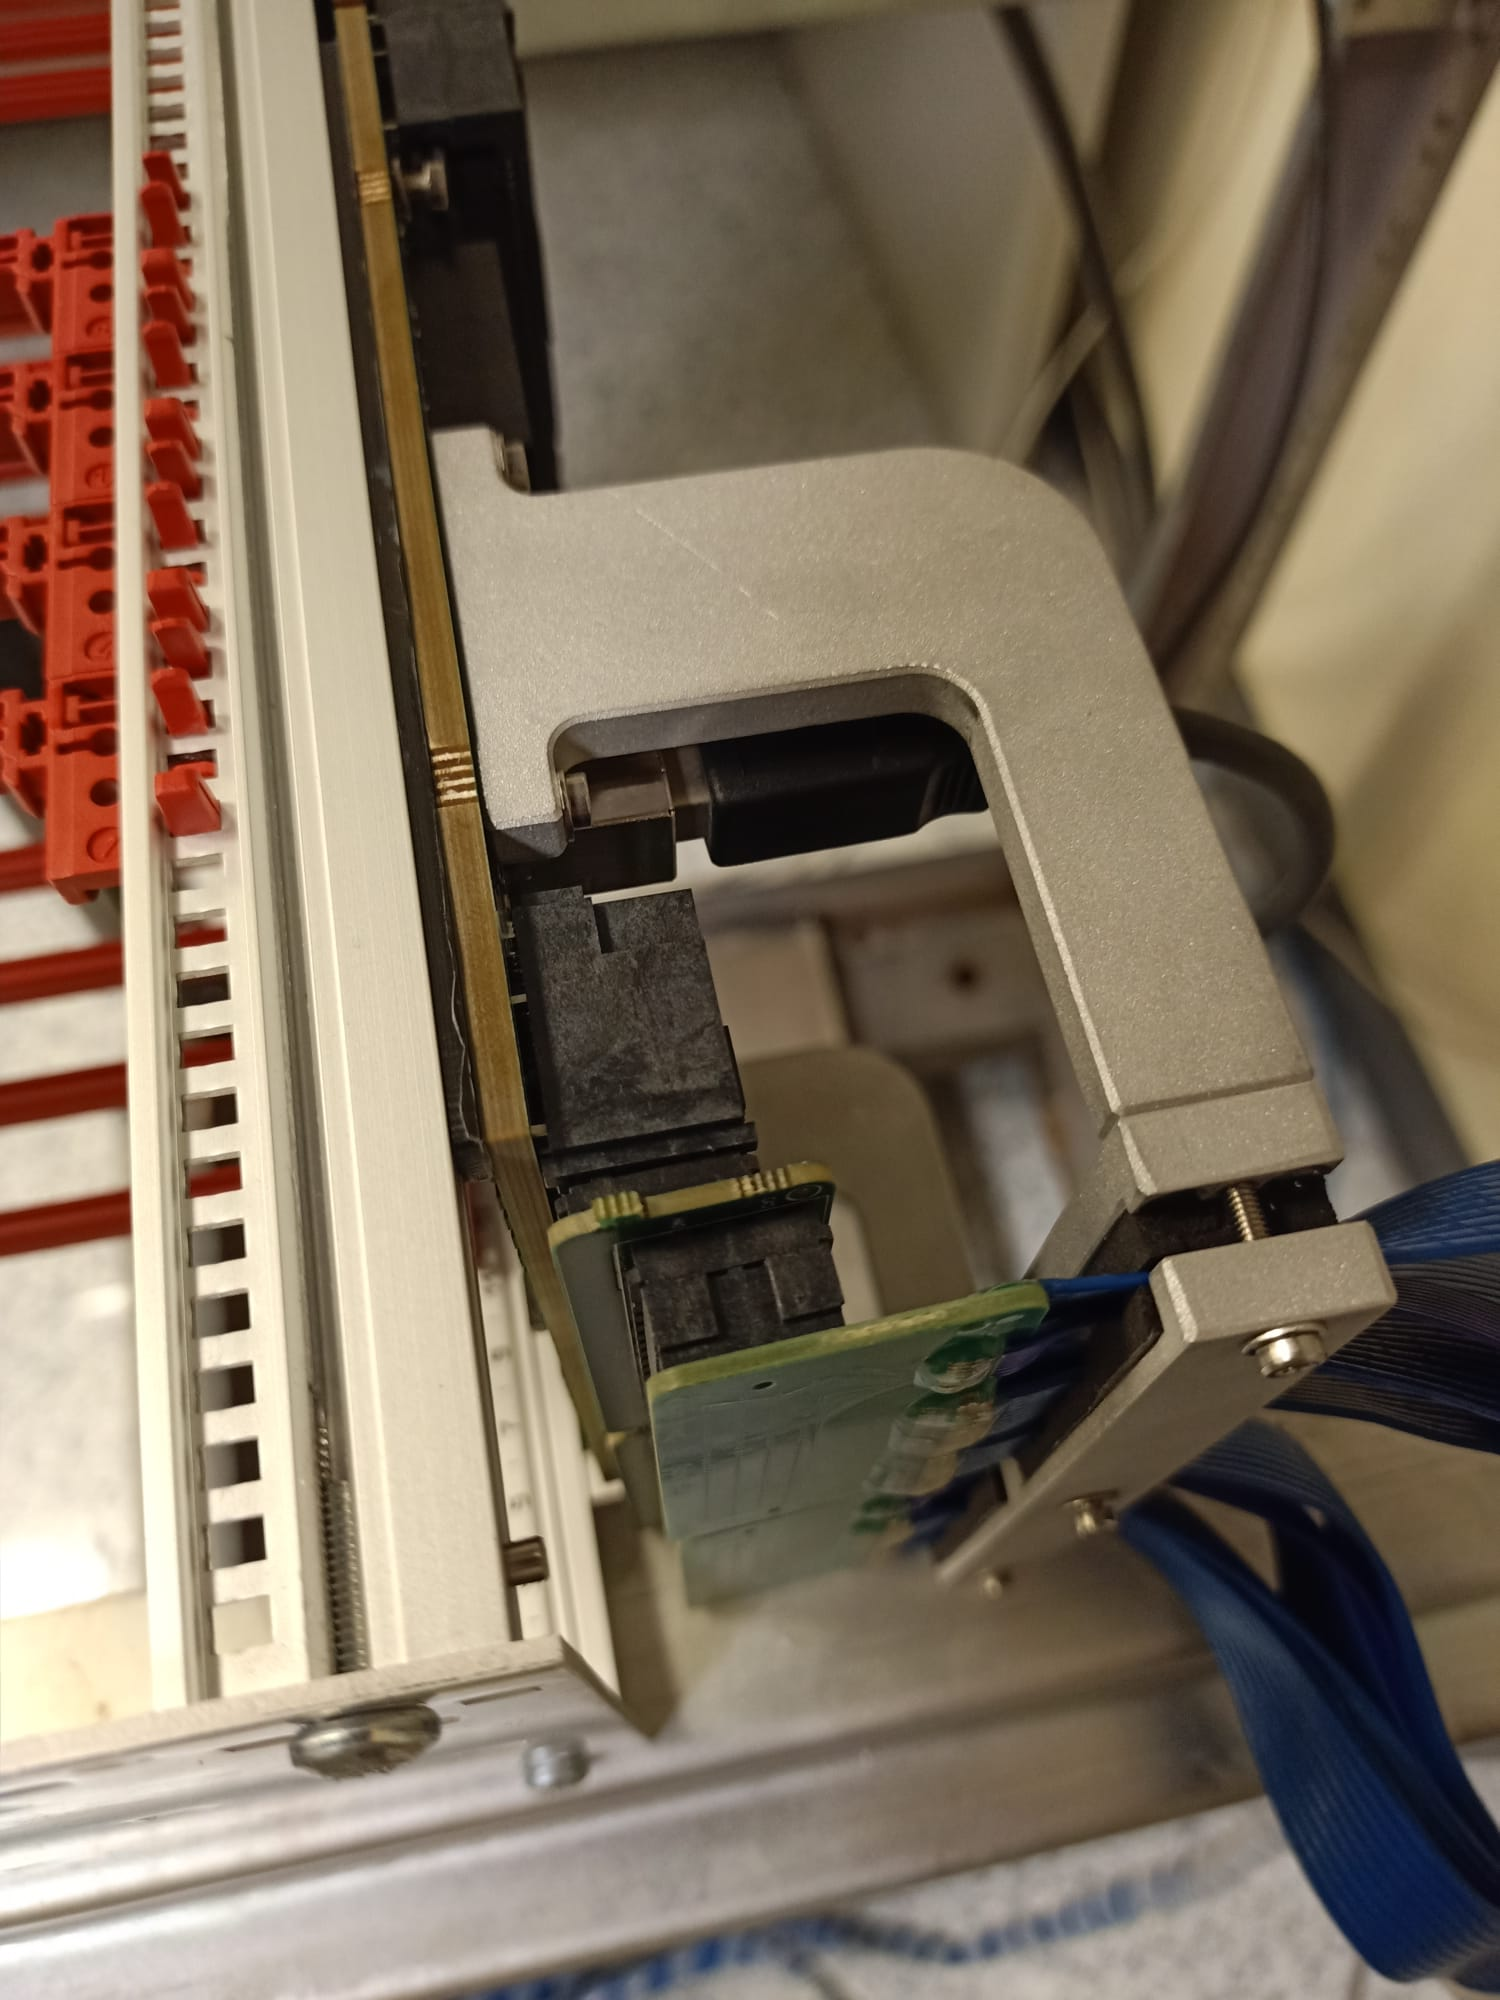
\includegraphics[width=0.4\linewidth]{FMC_Crate1.jpeg} 
  \caption{Picture of the connection of the FMC cable on the crate. The cables are secured using a long flat metalic piece with foam pad. The FMC adaptators are visible.}
  \label{FMC_Crate}
\end{figure}

\subsubsection{Usb cable connection}
The USB connection between the PC and the crate is achieved using a USB-A/USB-B cable. The USB-B plug is connected in the back of the first backplane (i.e. the closest to the FMC connectors) as shown in Figure \ref{USBBCrate}. 
Note that no usb device will be seen by the PC until a test card is correctly configured.

\begin{figure}[h!]
\centering
 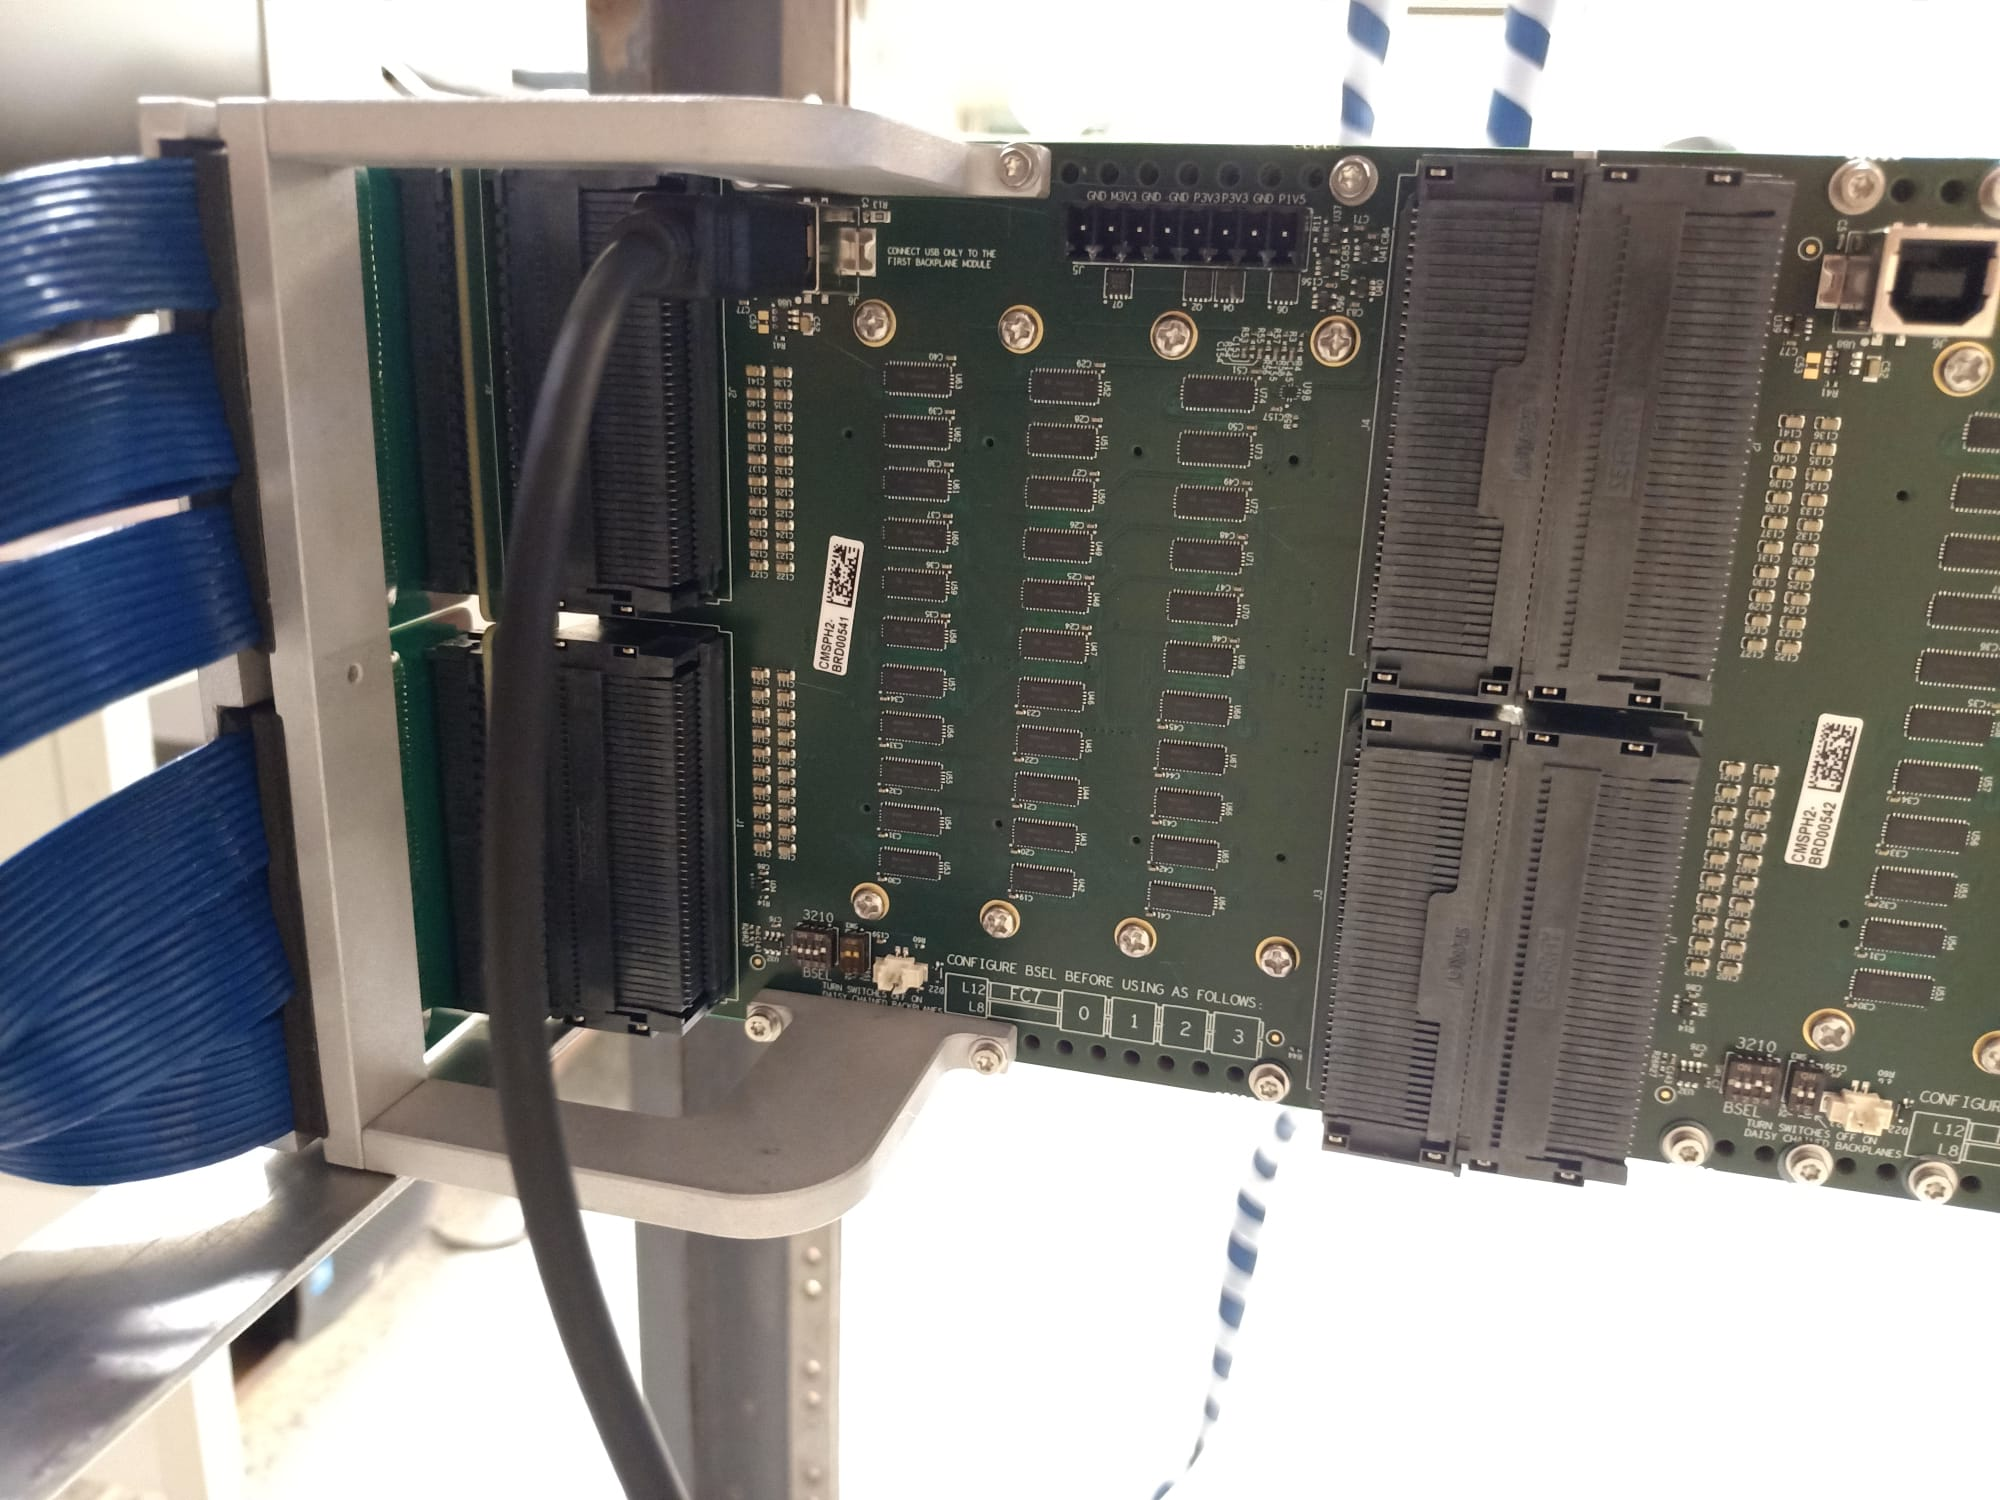
\includegraphics[width=0.8\linewidth]{USBBCrate.jpeg} 
  \caption{USB-B connection in the first backplane of the crate.}
  \label{USBBCrate}
\end{figure}

\subsection{AMC13 module}
In order to provide a clock to the system the AMC13 module can be used (\url{http://www.amc13.info}). The module can be plugged as in Figure \ref{amc13} and a loopback connection fiber must be plugged in. Note that even if the module is correctly powered no front panel led may be on.
\begin{figure}[h!]
\centering
 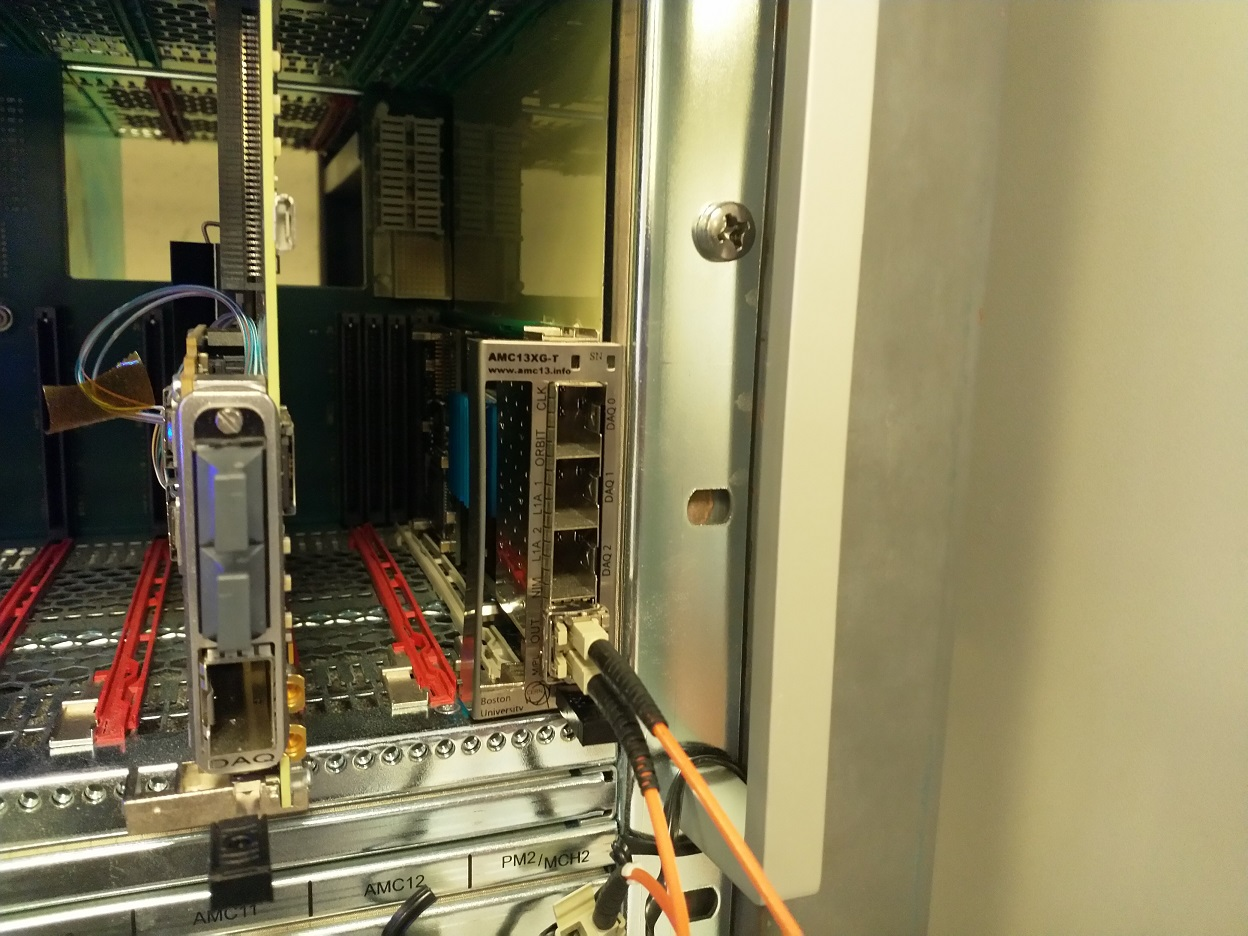
\includegraphics[width=0.8\linewidth]{amc13.jpg} 
  \caption{AMC13 module inside the crate.}
  \label{amc13}
\end{figure}




\section{PC setup and software installation}

The following instruction complete the following tutorials:
\url{https://cms-tracker-daq.web.cern.ch/cms-tracker-daq/tutorials/pc_connection/}.
Make sure the PC you use has two ethernet cards (enp1s0 and enp2s0). We will set the connection on enp1s0.

A few more details on how to prepare the FC7 and SD cards can be found here:
\url{https://cernbox.cern.ch/s/stFuUdRMdO7cxF6} or alternatively \url{https://www.ge.infn.it/~ferro/CMS/OTdocs/PreparingFC7-1.pdf}

Before proceeding install a rarp daemon as explained in \url{https://cms-tracker-daq.web.cern.ch/cms-tracker-daq/tutorials/pc_connection/}.

\subsection{Setting up the ethernet connection between the uTCA crate/FC7 and the PC} 
\label{fc7connection}
Once the rarp daemon has been installed and configured, do the following to verify the state of the enp1s0 interface and restart all the necessary services.
\begin{framed}
\begin{verbatim}
# Display the status of the ethernet interfaces of your PC
nmcli d 

# Restart the various ethernet services
sudo systemctl daemon-reload
sudo systemctl restart rarpd
sudo systemctl restart NetworkManager
\end{verbatim}
\end{framed}

Set an IP adress for the enp1s0 interface
\begin{framed}
\begin{verbatim}
#Check the IP adress of the ethernet interface
ifconfig 
#the inet field of enp1s0 where the uTCA crate is plugged should show an IP 
adress, otherwise do the following line to provide an IP adress to enp1s0
sudo ifconfig enp1s0 192.168.0.3  
\end{verbatim}
\end{framed}


The IP adress of the enp1s0 that we just configure as to be on the same network as the one of the FC7s. In other word with the enp1s0 adress set to 192.168.0.1, the IP adress of the FC7 have to be of the form 192.168.0.---

Also the subnet mask should be set to 255.255.0.0.

You can verify the state of the enp1s0 port using the following command:
\begin{framed}
\begin{verbatim}
# Verify that enp1s0 has state connected
nmcli d  
\end{verbatim}
\end{framed}
If the ethernet port is correctly configured, the following output will be displayed:
\begin{figure}[h!]
\centering
 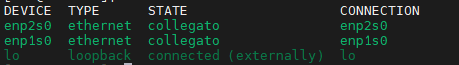
\includegraphics[width=0.6\linewidth]{Nmcli_output.png} 
  \caption{Screen display of the \emph{nmcli d} command if the enp1s0 port is well configured.}
  \label{GoodPing}
\end{figure}

In case, a FC7 is configured in the uTCA crate, one can "ping" it to verify the ethernet connection.
\begin{framed}
\begin{verbatim}
# ping an FC_7 if it is already installed
ping 'Name of your FC7'  
\end{verbatim}
\end{framed}
If the connection is established the output should look as in Figure \ref{GoodPing}, otherwise follow the instructions in the following section.


\subsection{Adding a new FC7 to the uTCA crate}
Switch off the uTCA crate, and plug the new FC7 in any available slot. Warning: to connect the FC7 it requieres a bit of force, make sure it is well plugged. If the following phase fails, first verify the FC7 connection.

Before switching on the crate, open a separate terminal and do:

\begin{framed}
\begin{verbatim}
tshark -i enp1s0  
\end{verbatim}
\end{framed}

This command listen to the enp1s0 interface and display all the packets going through it.
Now the uTCA crate on,  look for the broadcast of the newly connect FC7. It provides its MAC  adress. Note the MAC adress before proceeding.

\begin{framed}
\begin{verbatim}
#add a line in /etc/ethers with the MAC and a name for the FC7 (any you like)
sudo vim /etc/ethers 

#add a line in /etc/hosts with a IP adress and the corresponding name
sudo vim /etc/hosts  
\end{verbatim}
\end{framed}

The IP address of the new FC7 can be any address on the same sub-network as the ethernet port it is connected to : eg 192.168.0.---  in our case. Obviously, it also has to be different from addresses already used in $/etc/hosts $.

\begin{framed}
\begin{verbatim}
ping 'FC7 IP adress'
# or
ping 'FC7 name'
\end{verbatim}
\end{framed}

You should now be able to ping the new FC7. 

\begin{figure}[h!]
\centering
 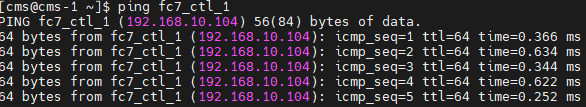
\includegraphics[width=0.8\linewidth]{PingResponse.png} 
  \caption{Screen display of the ping command if the FC7 has been well configured.}
  \label{GoodPing2}
\end{figure}

Files $/etc/hosts$ and $/etc/ethers$ should look like in Fig. \ref{GoodHosts}

\begin{figure}[h!]
\centering
%\begin{subfigure}[b]{0.475\textwidth}
  %      \centering
        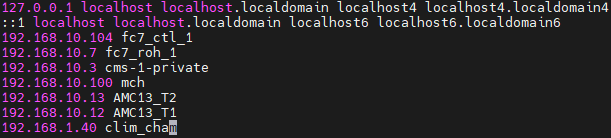
\includegraphics[width=\textwidth]{hosts.png}
    %\end{subfigure}
%\begin{subfigure}[b]{0.475\textwidth}
   %     \centering
        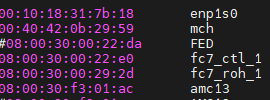
\includegraphics[width=0.5\textwidth]{ethers.png}
    %\end{subfigure}
  \caption{Screen display of /etc/hosts and /etc/ethers.}
  \label{GoodHosts}
\end{figure}




\subsection{Installing Ph2\_ACF}
Follow the instruction in \url{https://gitlab.cern.ch/cms_tk_ph2/Ph2_ACF}. 
The README provides straight forward tutorial to compile the code. On Alma9, follow the instruction in the \emph{"Setup on RHEL 9.1 or AlmaLinux 9.1"} section, and compile using the instruction in the \emph{"The Ph2\_ACF software"} section.

Be careful to install all the required packages. For what concerns {\it protobuf} package beware that during the checks (\emph{make check}) a big amount of memory is allocated, thus one of the checks can fail simply bacause of not enough available RAM.  

After cloning the repository, be sure to select the branch you want. See the available tags with \emph{git tag} and checkout the wished one with \emph{git checkout $<tagname>$}, like v4-14.


\subsection{Installing TCUsb}
Follow the instructions in \url{https://gitlab.cern.ch/cms_tk_ph2/cmsph2_tcusb}.
Once TCUsb has been compiled, you are asked to recompile \emph{Ph2\_ACF}. Before doing so, change line $127$ and $128$ of the \emph{Ph2\_ACF/setup.sh} file as:
\begin{framed}
\begin{verbatim}
export CompileWithTCUSB=true
\end{verbatim}
\end{framed}

Currently the TCUsb package used for POH tests is customized and downloadable from \url{https://gitlab.cern.ch/pszydlik/cmsph2_tcusb/-/tree/File_refactor?ref_type=heads}.

\subsection{Installing Powder (POH only)}
In order to use from remote the Power Supply during the test of POH's the Powder package must be installed \url{https://gitlab.cern.ch/cms_tk_ph2/power_supply}.
The config file must be properly modified:
\begin{framed}
\begin{verbatim}
File: config/configRohdeSchwartz.xml

<?xml version="1.0"? encoding="UTF-8"?>
<Devices>
    <PowerSupply
        ID          =   "PSU"
        InUse       =   "Yes"
        Model       =   "RohdeSchwarz"
        Connection  =   "Ethernet"
        IPAddress   =   "192.168.0.10"
        Port        =   "5025"
    >
    <Channel ID="P3V3"        Channel="2" InUse ="No" />
    <Channel ID="N3V3"        Channel="3" InUse ="No" />
    <Channel ID="TestVoltage" Channel="1" InUse ="Yes" />
    <Channel ID="Empty"       Channel="4" InUse ="No" />
    </PowerSupply>
</Devices>
\end{verbatim}
\end{framed}
Note that only the TestVoltage channel is remotely controlled. The other (2) channels must stay set as they are.

\par Before running the POH test the power supply server must be started on a new terminal window and left running till needed
\begin{framed}
\begin{verbatim}
PowerSupplyController -c config/configRohdeSchwartz.xml
\end{verbatim}
\end{framed}

\subsection{Installing Tc-controller}
The code can be downloaded from \url{https://gitlab.cern.ch/cms-ot-hybrids/tc-controller} and installed following the instructions in the README.
\par A config file must be added to define the test channel to be used by the controlled power supply.
In our case {\it config/configGenova.xml} has been edited accordingly to the setup in Powder package.

\subsection{Communicating with the FC7/Crate}

Never forget to set your command line to Ph2\_ACF dir and run the setup script \emph{. setup.sh} or \emph{source setup.sh}.

\subsubsection{Provide FC7 IP adress to the software}
To communicate with the FC7 using PH2\_ACF, you need to provide the IP adress of your FC7 to the program. This is done by changing the connection line in the xml description file (in our case \emph{settings/PS\_ROH.xml}) as:

\begin{framed}
\begin{verbatim}
 <connection id="board" uri="chtcp-2.0://localhost:10203?
 target='adress of your FC7':50001" 
 address_table="file://settings/address_tables/d19c_address_table.xml" />
\end{verbatim}
\end{framed}

and then do:
\begin{framed}
\begin{verbatim}
/opt/cactus/bin/controlhub_start
\end{verbatim}
\end{framed}

Note that if you have more than one FC7 board you need to provide a different (0, 1, 2, ...) board Id for each FC7.

\subsubsection{Writing the right firmware to the FC7 boards}
Firmware of the OT tracker can be download here: \url{https://udtc-ot-firmware.web.cern.ch/}
Someone should tell you which is the latest version of the firmware for your hw configuration.

\begin{framed}
\begin{verbatim}
#Go in Ph2_ACF folder
cd Ph2_ACF #or Ph2_ACF_Latest or others depending on the latest installed version

#Display the available firmware on the SD card of the FC7
fpgaconfig -b 'boardId' -c settings/PS_ROH.xml -l

#Upload firmware from the PC to the FC7 SD card
fpgaconfig -b 'boardId' -c settings/PS_ROH.xml 
-f 'firmware_file_name_on_the_PC.bin' 
-i 'firmware_name_on_the_microSD'

#for the electrical FC7 (the one with the blue falt cables)
fpgaconfig -b 1 -c settings/PS_ROH.xml -f FC7_firmwares/ps_roh_5g_electrical.bin 
-i ps_roh_5g_electrical

#for the optical FC7 (the one with the fibers)
fpgaconfig -b 0 -c settings/PS_ROH.xml -f ps_12m_5g_cic2_l12octa_l8quad.bin 
-i ps_12m_5g_cic2_l12octa_l8quad

#Upload a firmware of the FC7 fpga
fpgaconfig -b 0 -c settings/PS_ROH.xml -i  ps_12m_5g_cic2_l12octa_l8quad
fpgaconfig -b 1 -c settings/PS_ROH.xml -i ps_roh_5g_electrical
\end{verbatim}
\end{framed}

In case of {\bf POH} tests ONLY the electrical FC7 is used, since no data readout is needed. The boardId is in this case 0 (the HW settings can be just those in {\it settings/default.xml}) and there are two FWs that are used:
\begin{itemize}
\item[-] default\_LV.bin: used just to check for configurable cards in the mini-crate
\item[-] POH\_HV.bin: used to run the test (TestVoltage must be set to 10.5V to have it working properly)
\end{itemize}
 

\begin{figure}[h!]
\centering
 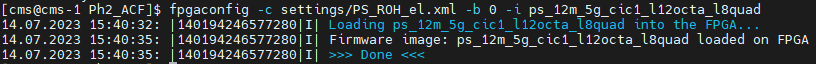
\includegraphics[width=\linewidth]{firmware-writing.png} 
  \caption{Screen display if the firmware has been correctly uploaded on the fpga}
\end{figure}

\subsubsection{Communication with the mini-crate and test boards}
First, a scan of the available test cards has to be done:
\begin{framed}
\begin{verbatim}
#Scan the crate, and display the slot occupied by a test card
mux_setup -f settings/PS_ROH.xml --mux_scan

#for POH
#mux_setup -f settings/default.xml --mux_scan 
\end{verbatim}
\end{framed}
From the output (see figure) one can see how many cards are connected to each backplane in which position.
\begin{figure}[h!]
\centering
 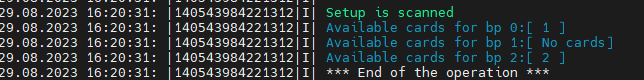
\includegraphics[width=\linewidth]{mux_scan.png} 
  \caption{Screen display after a crate scanning. Two test cards are found.}
\end{figure}
In order to configure the connection one can run 
\begin{framed}
\begin{verbatim}
#Configuring card 1 in backplane 0
mux_setup -f settings/PS_ROH.xml --mux_configure 0,1

#for POH
#mux_setup -f settings/default.xml --mux_configure 0,1
\end{verbatim}
\end{framed}
In order to setup the optical connection of the FC7 with the test card, one must identify the USB device via {\it lsusb} command looking for a line like
\begin{framed}
\begin{verbatim}
Bus 001 Device 005: ID 10c4:87a0 Silicon Labs PSRV2-CMSPH2-BRD00701 
\end{verbatim}
\end{framed}


\subsubsection{Using AMC13 clock}
In order to have more reliable results, the clock provided by the AMC13 module should be used, instead the internal one.
The AMC13 module should first set up and enabled. What follows has been extracted by the code and notes in gitlab repository at\\ \url{https://gitlab.cern.ch/cms-ot-hybrids/amc13-mch-configuration-scripts}.

First thing to do is to provide two IP adresses to the two tongues of the module T1 and T2. The procedure is the same as that used for adding a new FC7: use tshark to spot the MAC addresses of the two tongues and then edit /etc/ethers and /etc/hosts. The rule of thumb to identify T1 wrt T2 is that the one that keeps talking is T1. T1 and T2 IP addresses should differ by 1 digit (see Figure \ref{GoodHosts}).

In order to be able to configure the AMC13, one can have a look at \\
\url{https://gitlab.cern.ch/cms-ot-hybrids/amc13-mch-configuration-scripts/-/blob/master/Getting_started_with_AMC13_module.pdf?ref_type=heads} 
 (note that the instructions are for Centos7 and that some of the required packages may already be installed. Note also that the PATHs are sometimes referred to the home $\sim$ directory instead of the actual work dir. {\bf Forget} about the IP assignment algorithm unless strictly needed for some reason). 

After having installed the AMC13 code inside the amc13 dir, edit {\it connectionSN43.xml} with the right IPs and run 
\begin{framed}
\begin{verbatim}
. env.sh
tools/bin/AMC13Tool2.exe -c amc13/etc/amc13/connectionSN43.xml
\end{verbatim}
\end{framed}
If the AMC13 is connected no error will be reported and with the {\it list} command it will be shown as in Figure \ref{amc13connected}.
\begin{figure}[h!]
\centering
 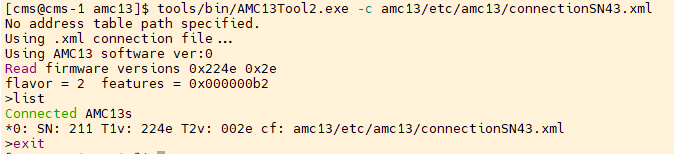
\includegraphics[width=\linewidth]{amc13connected.png} 
  \caption{Checking AMC13 connection.}
\label{amc13connected}
\end{figure}
In order to configure the AMC13 the following line can be entered instead of the {\it list} command:
\begin{framed}
\begin{verbatim}
> en 1-12 f t
> exit
\end{verbatim}
\end{framed}

The HW needs now to be instructed to use the clock provided by the AMC13 module. The file settings/PS\_ROH.xml needs to be modified setting the clock\_source\_u7 register to 0 for each board:
\begin{framed}
\begin{verbatim}
<Register name="clock_source_u7">0</Register>
\end{verbatim}
\end{framed}
a new file can be created (settings/PS\_ROH\_AMC.xml) and it can be used to configure the boards and rerun the test.


\subsection{Running the tests from command line}
The use of the GUI is recommended to run the tests. 
In order to run the test from command line for ROH's:
\begin{framed}
\begin{verbatim}
#device number should be checked with lsusb
#to check connectivity
PSROHTest -f settings/PS_ROH.xml -b --USBBus 1 --USBDev 5 

#run the full test
PSROHTest -f settings/PS_ROH.xml --ep 0xCA --test-fcmd --test-clock --test-i2c 1000 \
--test-eom --test-vtrx --test-reset --hybridId CMSPH2-PRT00193 -b \
--test-eom --measure-input-iv --USBBus 1 --USBDev 5
\end{verbatim}
\end{framed}
Note that all the optical channels are tested. At least one should be seen working.
If all the channels fail there is a problem in the transmission/receiving of the optical signal.\footnote[1]{FC7 version has to be checked.}
\footnote[2]{If an optical mezzanine is missing channel 0 might be seen as locked (!). Disable these channels to prevent errors.}

In order to run the test from command line for POH's:
\begin{framed}
\begin{verbatim}
pspoh_w_root_file -f ./config/configGenova.xml --useLoadVector \
--tc_File ./config/configPSPOH_short.xml --supplyStep 1 --supplyMin 8 \
--supplyMax 11 --hybridId PSPOH-210000001 --output PSPOH-210000001 \
--USBBus 1  --USBDev 095
\end{verbatim}
\end{framed}


\subsection{Installing and using the GUI}
In order to install the GUI, see the repository in gitlab \\
\url{https://gitlab.cern.ch/imateosd/gui-for-hybrids-testing-on-crate-systems}\\

The first time the GUI is used, the file hybrid/PSROH.py (or hybrid/PSPOH.py) might need to be updated. Especially the following variables:
\begin{itemize}
\item[-] PH2\_ACF\_WORKING\_DIRECTORY
\item[-] DESC\_FILES
\item[-] FIRMWARE
\end{itemize}

\begin{figure}[h!]
\centering
 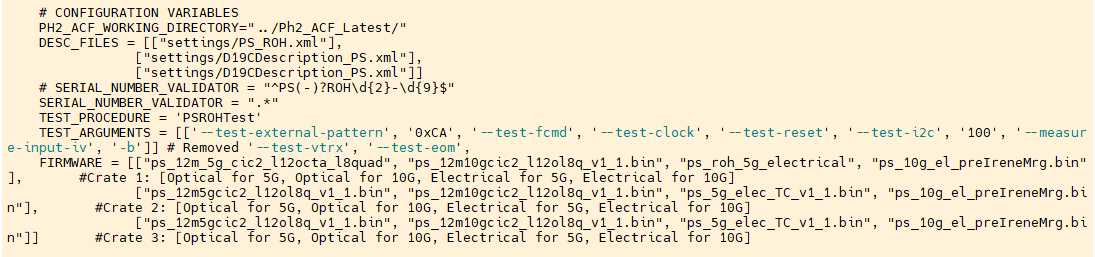
\includegraphics[width=\linewidth]{psroh.png} 
  \caption{Screen display of a portion of hybrid/PSROH.py}
  \label{screenshot}	
\end{figure}

configuration.json file must also be updated. Paths and test command name must be correctly specified (configurations for ROH and POH tests are of course different).
\begin{figure}[h!]
\centering
 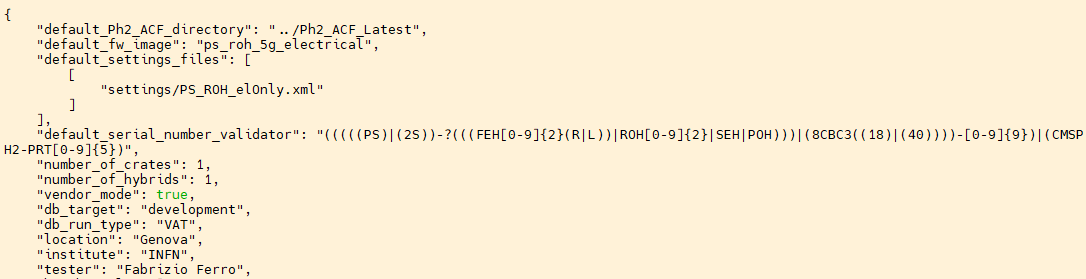
\includegraphics[width=\linewidth]{configuration.png} 
  \caption{Screen display of a portion of configuration.json for ROH test.}
\end{figure}

The following parameters need to be changed carefully:
\begin{itemize}
\item[-] default\_Ph2\_ACF\_directory : the directory where Ph2\_ACF is installed
\item[-] default\_fw\_image : the firmware image to be installed on the electrical FC7
\item[-] default\_settings\_files : a HW configuration xml file done on purpose where the electrical FC7 is board 0 (default.xml). 
\end{itemize}

CERN credential are requested the first time the GUI is run (or the cache reset). This is done to access the DB. For the moment being only SSO accounts are supported (no two factor authentication) that are registered to one of the following CERN e-groups:
\begin{itemize}
\item[-] Construction Operator: cms-tracker-assemblyOperators
\item[-] Quality Control Operator: cms-tracker-qcOperators
\item[-] Tracking Operator: cms-tracker-trackingOperators
\end{itemize}
The access is granted only to the {\it production} DB and not to the {\it development} one (see configuration.json). For more information:
\url{https://espace.cern.ch/Tracker-Upgrade/DataBase/SitePages/Home.aspx}.

The commands to run the GUI are:

\begin{framed}
\begin{verbatim}
#inside gui-for-hybrids-testing-on-crate-systems
source setup.sh
python3 cratetesting.py
\end{verbatim}
\end{framed}

The GUI will ask how many hybrid one wants to test and to insert the full code (bar code) of test card and hybrid module.
No character will be typed if different from expected (e.g. usually names start with CMSPH2). \\
When the button to run the test is pushed, the GUI will first check for the presence of the boards in the mini-crate and then actually run the test. \\

When the test is finished, at least one Enter command must be typed in the terminal window to complete the DB upload procedure. It typically fails despite messages of success are displayed. 

\newpage

\appendix

\appendixpage
\section{Original instruction files}

\includepdf[pages=-]{./Includes/PS-POH_instructions_to_run_tests.pdf}
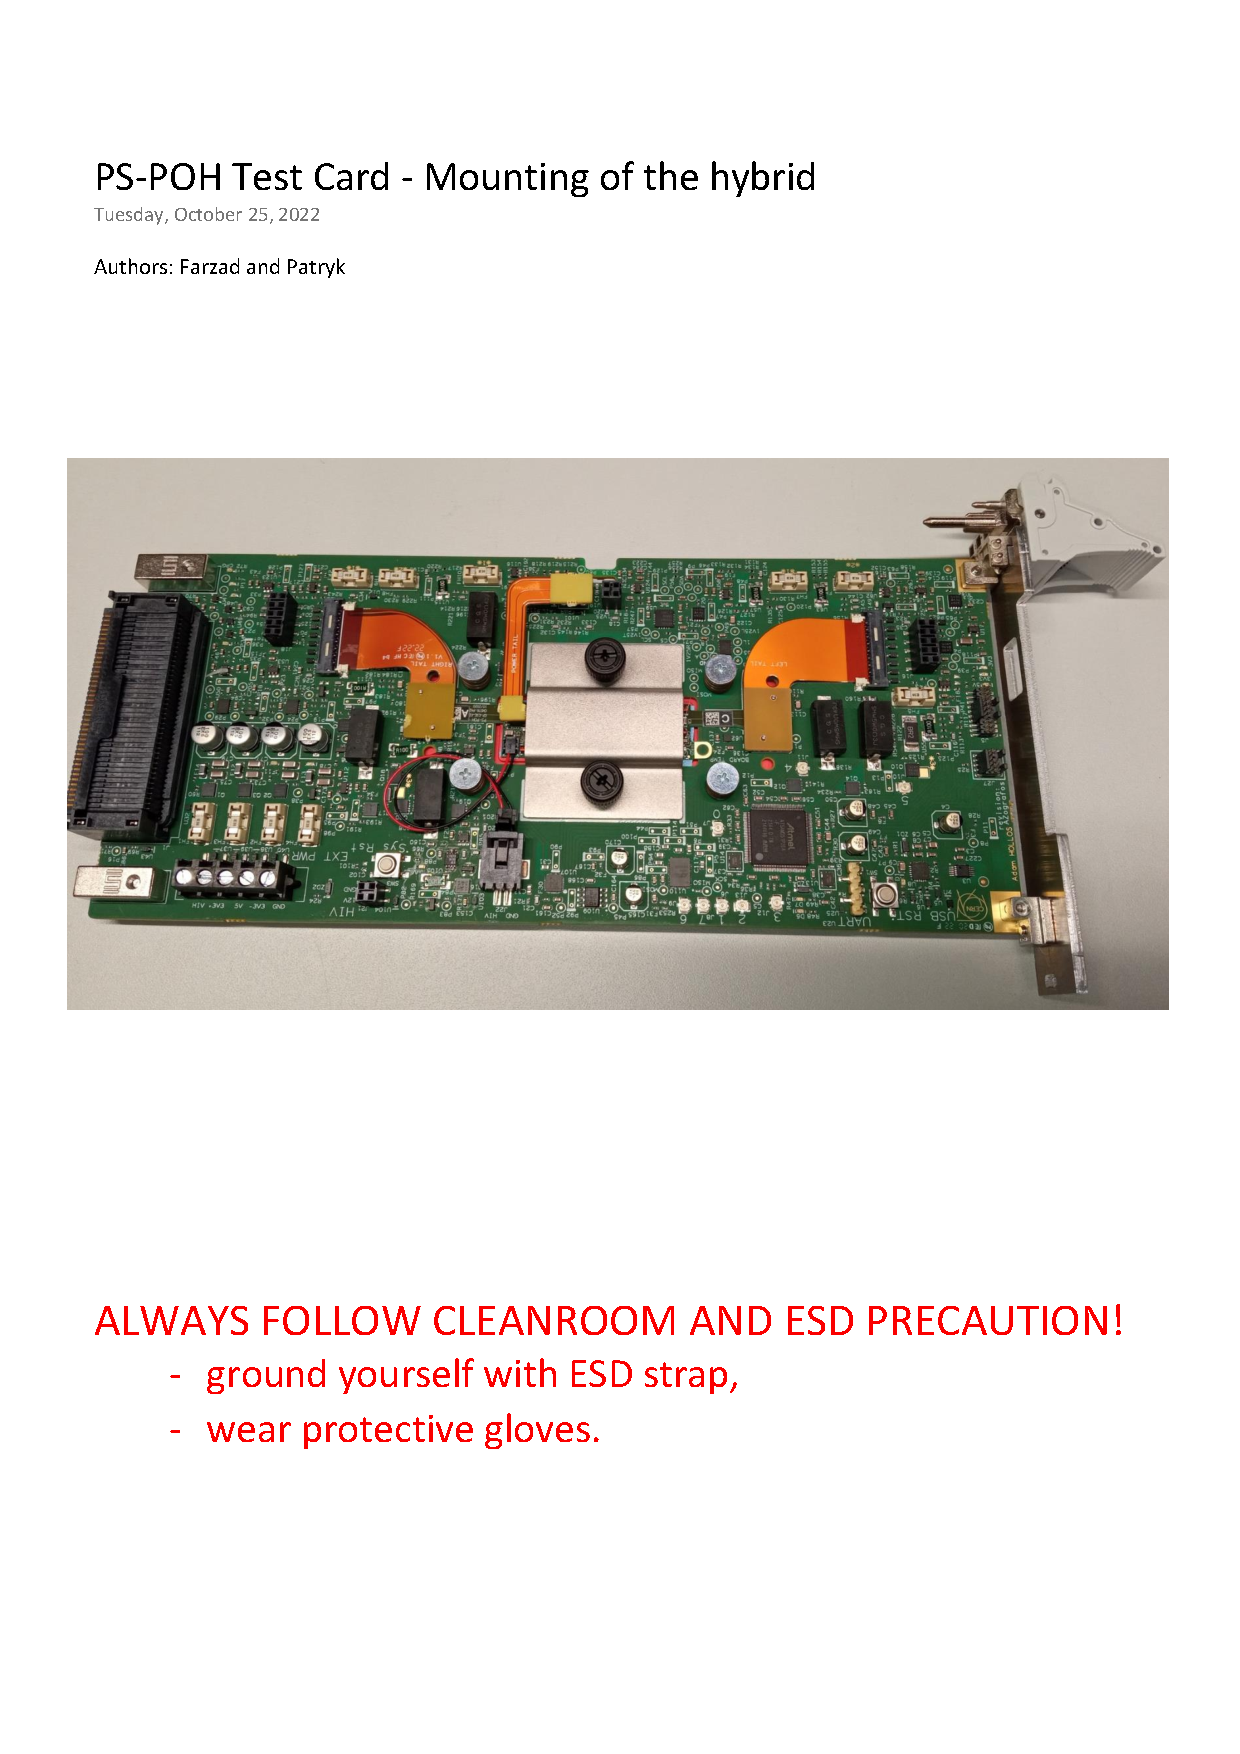
\includepdf[pages=-]{./Includes/PS-POH_mounting_guide.pdf}


\end{document}